\documentclass[11pt,a4paper]{article}
% Real word spaces and Unicode glyph names in the PDF, so that text extracted
% from it (search, copy, automated readers) matches the typeset text.
\input{glyphtounicode}
\pdfgentounicode=1
\pdfinterwordspaceon
\usepackage[utf8]{inputenc}
\usepackage[T1]{fontenc}
\usepackage{lmodern}
\usepackage{amsmath,amssymb,amsthm,mathtools}
\usepackage{booktabs}
\usepackage{graphicx}
\usepackage{microtype}
\usepackage{xurl}
\emergencystretch=1.5em
\usepackage[margin=2.5cm]{geometry}
\usepackage[hidelinks]{hyperref}

\newtheorem{theorem}{Theorem}
\newtheorem{lemma}[theorem]{Lemma}
\newtheorem{proposition}[theorem]{Proposition}
\newtheorem{corollary}[theorem]{Corollary}
\theoremstyle{definition}
\newtheorem{definition}[theorem]{Definition}
\newtheorem{assumption}{Assumption}
\theoremstyle{remark}
\newtheorem{remark}[theorem]{Remark}

\newcommand{\R}{\mathbb{R}}
\newcommand{\dH}{d_{\mathrm{H}}}
\newcommand{\dist}{\operatorname{dist}}
\newcommand{\conv}{\operatorname{conv}}
\newcommand{\seg}[2]{[#1,#2]}
\newcommand{\ip}[2]{\langle #1,#2\rangle}

\title{Certified Raster-to-Curve Conversion:\\
Verified Hausdorff Bounds, Topology Certificates and\\
Provably Minimal Polygons for Binary Shapes}
\author{Hakan Karateke}
\date{Draft --- \today}

\begin{document}
\maketitle

\begin{abstract}
Raster-to-vector tools return curves whose distance to the input and whose
topology are, at best, measured by sampling. We study the constrained problem
\emph{minimise description cost subject to a two-sided Hausdorff error at most
$\varepsilon$ and an unchanged planar topology} for the pixel boundary of a
binary image, and we attach to every answer a certificate that an independent
checker re-derives from the stored coefficients alone. The checker interprets
binary64 coefficients as exact dyadic rationals, subdivides polynomial and
positive-weight rational B\'ezier pieces in exact arithmetic, and bounds all
distances with outward-rounded intervals. Topology is established by rational
sufficient conditions (chord-monotone leaves, separating lines, disjoint convex
hulls, equal nesting forests) or, for boundaries with point contacts, by a
replayable empty-triangle witness. For the polygonal family we compute a
\emph{provably minimal} node-restricted polygon with a ray-wedge shortest-cycle
algorithm whose answer is re-verified exactly. On the 2050 glyphs of an
MIT-licensed icon set and four tolerances (8200 instances) the
Ramer--Douglas--Peucker heuristic uses a median $2.8$ times, and on single
inputs more than thirty times, the minimal number of edges at a tolerance of
one pixel. A joint,
contact-preserving formulation, solved exactly by conflict-driven branch and
bound and certified by a new exact criterion for touching rings, is proven
optimal and certified on all 8200 instances. The same shortest-cycle
argument is extended to rings of line segments and circular arcs: the bulges
for which an arc stays within the tolerance of a node form an interval with
closed-form end points, which gives a provably minimal node-restricted
line--arc ring, proven minimal on all 800 sampled instances with $30$--$66\%$
of the edges of the minimal polygon. The full pipeline returns a proven model
on all 800 sampled runs. Potrace~1.16, measured against the same reference,
exceeds one pixel of error on all but 4 of the 2050 inputs with curve
smoothing and changes the component or hole count on about $4.9\%$ of them;
attached to Potrace's output, the same checker proves $1859$ of the 2050
results correct to two pixels. All inputs are processed at their own
resolution: resampling to a fixed plane, as earlier versions did, changes the
topology of thin-line drawings drastically. The minimal polygon and its
certificate scale to a $67$-megapixel contour-like input, and flat-colour
images are handled as stacked binary layers, each with its own certificate.
\end{abstract}

\section{Introduction}

Converting a bilevel raster shape into a short list of parametric pieces is a
classical task~\cite{selinger2003potrace,schneider1990fitting,kopf2011depixelizing}
that is now mostly approached with perceptual models~\cite{dominici2020} and
learned generators~\cite{rodriguez2025,gehlaut2026}.
These methods optimise visual quality and report no guarantee about how far
the output is from the input or whether holes, components and their nesting
survive. When the output feeds a downstream geometric pipeline (CAD profiles,
machining, measurement) these two properties are the specification.

We take the \emph{pixel boundary} $\Gamma$ of the thresholded image as the
reference object. It is a finite union of axis-parallel segments with integer
vertices, so it can be represented without loss. The task is
\begin{equation}\label{eq:problem}
  \min_{M\in\mathcal{M}} C(M)\quad\text{subject to}\quad
  \dH(\Gamma,M)\le\varepsilon,\qquad M\simeq\Gamma ,
\end{equation}
where $\mathcal{M}$ is a family of piecewise parametric closed curves, $C$ a
description cost and $\simeq$ equality of planar topology
(Definition~\ref{def:topology}). We make no claim about an ideal continuous
shape behind the raster; accuracy statements concern $\Gamma$ only.

\paragraph{Contributions.}
\begin{enumerate}
\item A \emph{certified error bound} (Theorem~\ref{thm:hausdorff}): an upper
  bound $U\ge\dH(\Gamma,M)$ computed with exact rational subdivision and
  outward-rounded interval arithmetic, valid for lines, cubic B\'ezier and
  B-spline pieces, positive-weight rational conic arcs and full
  circles/ellipses.
\item \emph{Topology certificates}: rational sufficient conditions that prove
  each model ring is a Jordan curve, rings are pairwise disjoint and the nesting
  forest equals that of $\Gamma$ (Theorem~\ref{thm:jordan},
  Corollary~\ref{cor:isotopy}); and an empty-triangle witness for references
  with point contacts (Theorem~\ref{thm:triangle}).
\item A \emph{provably minimal node-restricted polygon}
  (Theorem~\ref{thm:minlink}) with a certified lower bound, giving the first
  optimality-gap measurements for the heuristic stages of the pipeline, and a
  resolution statement explaining when sub-pixel tolerances cannot compress a
  staircase (Proposition~\ref{prop:staircase}).
\item A \emph{contact-preserving joint optimum} (Theorem~\ref{thm:bnb}): the
  minimum total number of edges over all rings subject to pinned contact
  points and pairwise clearance, computed exactly by conflict-driven
  branch and bound although simple minimum-link simplification is NP-hard in
  general; and an \emph{exact certificate for touching rings}
  (Theorem~\ref{thm:contact}) that needs neither sampling nor intervals.
\item A \emph{provably minimal node-restricted line--arc ring}
  (Theorem~\ref{thm:arcs}), based on the observation that the admissible
  bulges of an arc through two fixed nodes form an interval with closed-form
  end points (Proposition~\ref{prop:interval}); it extends the optimality
  statement from polygons to a curved family that the certificate already
  covers.
\item An open implementation whose project files are re-certified on load, and
  an evaluation on 2050 inputs including an independent audit of Potrace, the
  certification of Potrace's own output by the same checker, runs at native
  resolution up to $67$ megapixels, and flat-colour inputs treated as stacked
  certified layers.
\end{enumerate}

\section{Related work}

\emph{Classical tracing.} Potrace~\cite{selinger2003potrace} builds an optimal
polygon under its own straightness criterion and then smooths corners with
B\'ezier segments; Schneider~\cite{schneider1990fitting} fits cubics by least
squares with reparameterisation; Kopf and
Lischinski~\cite{kopf2011depixelizing} target pixel art.

\emph{Perception-driven vectorisation.} Hoshyari et al.~\cite{hoshyari2018} and
PolyFit~\cite{dominici2020} choose corners and primitives with learned
perceptual models and validate the output by user studies; PolyFit, like the
present work, passes through an intermediate polygon, selected there for
perceptual plausibility and here for provable minimality. The objective of
this line is agreement with human expectation; no bound on the distance to
the raster boundary is stated.

\emph{Learning-based vectorisation.} Differentiable
rasterisation~\cite{li2020diffvg} made image-space optimisation of paths
possible; layer-wise optimisation~\cite{ma2022}, superpixel-based
synthesis~\cite{hu2024} and, most recently, vision--language models that emit
SVG code~\cite{rodriguez2025,gehlaut2026} followed. These methods are
evaluated by pixel or perceptual losses on a rendering of the output. Their
output carries no statement about $\dH$ to the input boundary or about
topology, and a rendering loss cannot provide one: a thin crossing between two
rings changes the planar topology at negligible pixel cost. Our certificates
are orthogonal to the generator and could in principle be attached to the
output of any of these methods.

\emph{Variational and topology-aware vectorisation.} He, Kang and
Morel~\cite{he2023,he2024} vectorise by affine scale-space smoothing and
region merging and give bounds guaranteeing that the topology of the
\emph{region partition} is consistent; Chen and Peng~\cite{chen2024} downsample
binary images while provably preserving Betti numbers. Both guarantee
topology, neither bounds the two-sided Hausdorff error of a parametric model,
and neither issues a certificate that can be re-checked from the stored
output.

\emph{Curve simplification.} The Ramer--Douglas--Peucker
heuristic~\cite{ramer1972,douglas1973} gives no minimality. The min-\# problem
of Imai and Iri~\cite{imai1988} asks for the fewest vertices such that every
shortcut is within tolerance of the sub-chain it replaces, and is solved as a
shortest path in a shortcut graph; Chan and Chin~\cite{chan1996} construct that
graph in quadratic time. This \emph{local} criterion must be distinguished from
the \emph{global} one, $\dH(\Gamma,Q)\le\tau$ for the whole curve: van Kreveld,
L\"offler and Wiratma~\cite{vankreveld2018} showed that minimising the number
of vertices under the global undirected Hausdorff distance is NP-hard, while
the global Fr\'echet variant is polynomial~\cite{vankreveld2018,bringmann2019};
the landscape for further vertex restrictions and distance variants is charted
in~\cite{vandekerkhof2019}. Unrestricted minimum-link variants are studied
in~\cite{guibas1993,agarwal2005}, where requiring a simple output is already
NP-hard~\cite{guibas1993}. For digital curves, Sivignon~\cite{sivignon2014}
gives a near-linear simplification with a guaranteed Fr\'echet error but no
minimality. We solve the local problem exactly on closed pixel boundaries
(Theorem~\ref{thm:minlink}); by Proposition~\ref{prop:capsule-chain} its
solutions are feasible for the global constraint, and the hardness results
explain why we neither claim global optimality nor build simplicity into the
search. Topologically consistent simplification of subdivisions goes back to
de~Berg et al.~\cite{deberg1998}; our empty-triangle witness is a
vertex-removal rule in that tradition, made replayable in exact arithmetic.

\emph{Certified geometry.} Isotopic approximation of implicit curves by
interval subdivision~\cite{plantinga2004} is the closest methodological
relative; we treat the parametric, piecewise case with a discrete reference.
Interval arithmetic follows~\cite{moore2009}; B\'ezier and NURBS facts
follow~\cite{farin2002,piegl1997}.

\section{Setting}

Let $\Gamma=\bigcup_{i=1}^{r}\Gamma_i$, where each ring $\Gamma_i$ is a closed
polygonal chain with integer vertices obtained by tracing the edges of the
foreground unit squares (4-connectivity for the foreground) and merging
collinear edges. A model is $M=\bigcup_{i=1}^{r}M_i$, each $M_i$ a closed
concatenation of \emph{pieces}: segments, cubic B\'ezier curves, cubic
B-spline spans, rational quadratic arcs
$r(u)=\frac{(1-u)^2A+2u(1-u)wP+u^2B}{(1-u)^2+2wu(1-u)+u^2}$ with $w>0$, or one
full circle/ellipse. For compact $A,B\subset\R^2$,
$\vec d(A,B)=\max_{a\in A}\dist(a,B)$ and
$\dH(A,B)=\max\{\vec d(A,B),\vec d(B,A)\}$.

\begin{definition}[Planar topology]\label{def:topology}
Two families of pairwise disjoint Jordan curves $(\Gamma_i)_i$, $(M_i)_i$ with
the same index set have the same planar topology, $M\simeq\Gamma$, if for all
$i\ne j$ the curve $M_i$ lies inside $M_j$ exactly when $\Gamma_i$ lies inside
$\Gamma_j$, and $M_i$, $\Gamma_i$ have the same orientation.
\end{definition}

\begin{assumption}[Arithmetic]\label{ass:ieee}
Stored coefficients are finite binary64 numbers, read as exact dyadic
rationals. The operations $+,-,\times,\div,\sqrt{\cdot}$ on binary64 are
correctly rounded as in IEEE~754~\cite{ieee754}, with gradual underflow and
without value-changing reassociation.
\end{assumption}

\begin{lemma}[Outward rounding]\label{lem:outward}
Under Assumption~\ref{ass:ieee}, if $\tilde z$ is the computed result of a
basic operation with exact result $z$, then
$z\in[\operatorname{pred}(\tilde z),\operatorname{succ}(\tilde z)]$. Hence
interval operations that widen each computed endpoint by one unit in the last
place enclose the exact range.
\end{lemma}
\begin{proof}
Correct rounding returns a floating-point neighbour of $z$ (or $z$ itself), so
$z$ lies between the predecessor and successor of $\tilde z$. Enclosure of
compound expressions follows by induction over the expression tree, using
monotonicity of each endpoint formula.
\end{proof}

\section{Certified error bound}

\begin{lemma}[Chord capsule]\label{lem:capsule}
Let $c:[0,1]\to\R^2$ be continuous with $c(0)=a\ne b=c(1)$ and
$c([0,1])\subset\conv(K)$ for a finite set $K$. If
$\dist(k,\seg ab)\le\delta$ for all $k\in K$, then
$\dH\bigl(c([0,1]),\seg ab\bigr)\le\delta$.
\end{lemma}
\begin{proof}
The capsule $N=\{x:\dist(x,\seg ab)\le\delta\}$ is convex and contains $K$,
hence $\conv(K)$ and the curve; this bounds $\vec d(c,\seg ab)$. Conversely let
$u=(b-a)/\lVert b-a\rVert$ and $f(t)=\ip{c(t)-a}{u}$. Then $f$ is continuous
with $f(0)=0$, $f(1)=\lVert b-a\rVert$, so for every
$q=a+su\in\seg ab$ there is $t$ with $f(t)=s$. The point $c(t)\in N$ projects
orthogonally onto $q\in\seg ab$, so its nearest point on the line through
$a,b$ is $q$ and $\lVert c(t)-q\rVert=\dist(c(t),\seg ab)\le\delta$.
\end{proof}

Polynomial B\'ezier curves lie in the convex hull of their control points; so
do rational B\'ezier curves with positive weights, whose basis functions
$w_iB_i^n(u)/\sum_jw_jB_j^n(u)$ are non-negative and sum to
one~\cite{farin2002,piegl1997}. De~Casteljau subdivision at $u=\tfrac12$, in
homogeneous coordinates for the rational case, is exact over the rationals and
preserves positivity of weights. Subdividing until every leaf satisfies the
hypothesis of Lemma~\ref{lem:capsule}, with distances bounded from above by
interval arithmetic and with the binary64 rounding error of the leaf endpoints
added, yields for each ring a polygon $P_i$ and a number $\delta_i$ with
$\dH(M_i,P_i)\le\delta_i$. Cubic B-spline spans are first converted to
B\'ezier form by exact rational evaluation of the end values and derivatives.

\begin{lemma}[Sampling]\label{lem:sampling}
Let $A$ be a finite union of segments and $S\subset A$ a finite set containing
all segment endpoints such that consecutive samples on each segment are at
most $h$ apart. For any compact $B$ and any choice of a \emph{witness} segment
$e_s\subset B$ for each $s\in S$,
\[
  \vec d(A,B)\le\max_{s\in S}\dist(s,e_s)+\tfrac h2 .
\]
\end{lemma}
\begin{proof}
Every $a\in A$ has a sample $s$ on its segment with $\lVert a-s\rVert\le h/2$.
Since $x\mapsto\dist(x,B)$ is $1$-Lipschitz and
$\dist(s,B)\le\dist(s,e_s)$, the claim follows.
\end{proof}

The witness need not be the nearest segment: any segment gives a valid upper
bound, so a floating-point spatial index may propose witnesses without entering
the trusted base.

\begin{theorem}[Certified Hausdorff bound]\label{thm:hausdorff}
Let $P_i,\delta_i$ be as above, let $S_i\subset\Gamma_i$ and $T_i\subset P_i$
be sample sets with spacing at most $h$, and let $d_i^{+}$ be an upper bound
for both $\max_{s\in S_i}\dist(s,e_s)$ with witnesses $e_s\subset P_i$ and
$\max_{t\in T_i}\dist(t,e_t)$ with witnesses $e_t\subset\Gamma_i$. Then
\[
  \dH(\Gamma,M)\;\le\;U:=\max_i\bigl(d_i^{+}+\tfrac h2+\delta_i\bigr).
\]
Under Assumption~\ref{ass:ieee} the value computed with outward-rounded
intervals is at least $U$.
\end{theorem}
\begin{proof}
By Lemma~\ref{lem:sampling} applied in both directions,
$\dH(\Gamma_i,P_i)\le d_i^{+}+h/2$. The triangle inequality for $\dH$ and
$\dH(P_i,M_i)\le\delta_i$ give $\dH(\Gamma_i,M_i)\le d_i^{+}+h/2+\delta_i$.
Finally $\dH(\bigcup_iA_i,\bigcup_iB_i)\le\max_i\dH(A_i,B_i)$. The last
sentence is Lemma~\ref{lem:outward}.
\end{proof}

\begin{remark}
$U$ bounds the distance between the stored model and the stored reference. It
says nothing about the quality of the fit that produced the coefficients, about
RMS error or about area; those remain sampled diagnostics.
\end{remark}

\section{Topology certificates}

\subsection{Jordan rings by rational sufficient conditions}

Let ring $i$ be subdivided into leaves $L^i_1,\dots,L^i_{N_i}$ in cyclic order,
each a (rational, positive-weight) B\'ezier curve with control points
$c_0,\dots,c_n$ and chord vector $d=c_n-c_0$.

\begin{theorem}[Simple disjoint rings]\label{thm:jordan}
Suppose that for every ring $N_i\ge3$ and
\begin{enumerate}
\item[(i)] \emph{chord monotonicity}: $d\ne0$ and
  $\ip{c_{k+1}-c_k}{d}\ge0$ for $k=0,\dots,n-1$, for every leaf;
\item[(ii)] \emph{adjacent separation}: consecutive leaves $L,L'$ of a ring
  share the endpoint $p=c_n=c'_0$ exactly, and there is a vector $\nu$ with
  $\ip{c_k-p}{\nu}\le0$ for all $k$, $\ip{c'_k-p}{\nu}\ge0$ for all $k$,
  $\ip{c_0-p}{\nu}<0$ and $\ip{c'_n-p}{\nu}>0$;
\item[(iii)] \emph{hull separation}: any two leaves that are not consecutive in
  the same ring have disjoint convex hulls of control points.
\end{enumerate}
Then every $M_i$ is a Jordan curve, the $M_i$ are pairwise disjoint, and the
same holds for the chord polygons $P_i$. Moreover $M$ and $P$ have the same
planar topology.
\end{theorem}
\begin{proof}
\emph{Leaves are injective.} For a polynomial leaf,
$g(u)=\ip{c(u)-c_0}{d}$ has derivative
\[
  g'(u)=n\sum_kB^{n-1}_k(u)\,\ip{c_{k+1}-c_k}{d}.
\]
The coefficients are non-negative and
sum to $\lVert d\rVert^2>0$, so at least one is positive and $g'>0$ on $(0,1)$.
For a rational leaf write $c(u)=\sum_kp_k(u)c_k$ with
$p_k\propto w_k\binom nku^k(1-u)^{n-k}$; then
\[
  g(u)=\sum_kp_k(u)\,s_k,\qquad
  g'(u)=\frac{\operatorname{Cov}_{p(u)}(s_k,k)}{u(1-u)},
\]
where $s_k=\ip{c_k-c_0}{d}$ is non-decreasing in $k$ by (i). The covariance of two
non-decreasing functions of $k$ under a distribution with full support is
non-negative, and positive because $s_0<s_n$. In both cases $g$ is strictly
increasing, hence $c$ is injective.

\emph{Consecutive leaves meet only at $p$.} For $u<1$ the point $c(u)$ is a
convex combination of the $c_k$ with positive weight on $c_0$, so
$\ip{c(u)-p}{\nu}<0$; symmetrically $\ip{c'(u)-p}{\nu}>0$ for $u>0$.

\emph{Other leaves are disjoint} by (iii) and the convex hull property. Since
$N_i\ge3$, each $M_i$ is a closed curve without self-intersection, and distinct
rings are disjoint.

\emph{Deformation to the chord polygon.} Parametrise the chord of a leaf by
$\ell(u)=c_0+\frac{g(u)}{\lVert d\rVert^2}d$ and set
$H_s(u)=(1-s)c(u)+s\,\ell(u)$, $s\in[0,1]$. Then
$\ip{H_s(u)-c_0}{d}=g(u)$ for all $s$, so each deformed leaf stays injective; it
stays in the convex hull of the control points, so (iii) keeps non-consecutive
leaves apart; and $\ell(u)$ for $u<1$ is a convex combination of $c_0$ and $p$
with positive weight on $c_0$, so the strict inequalities of the previous
paragraph persist. Hence $(H_s)_s$ is a continuous family of embeddings of the
disjoint union of $r$ circles joining $M$ to $P$. Along such a family the
winding number of ring $i$ around a point of ring $j$ is a continuous integer,
hence constant, so containment relations and orientations agree for $M$ and
$P$.
\end{proof}

All quantities in (i)--(iii) are signs of rational expressions and are decided
exactly. In (ii) the vector $\nu$ is proposed in floating point (the bisector
of the two chords) and then converted to a rational, so that the inequalities
are checked exactly for that $\nu$; in (iii) a separating axis is searched
among the hull edge normals.

\begin{corollary}[Certified topology]\label{cor:isotopy}
If the leaves of $M$ and the edges of $\Gamma$ both satisfy
Theorem~\ref{thm:jordan}, and the nesting forests and orientations of $P$ and
$\Gamma$, computed with exact signed areas and exact ray crossing, coincide,
then $M\simeq\Gamma$. Consequently there is an orientation-preserving
homeomorphism of the plane, isotopic to the identity, carrying each $\Gamma_i$
to $M_i$.
\end{corollary}
\begin{proof}
The first statement combines Theorem~\ref{thm:jordan} for $M$ with the exact
comparison. The second is the classical consequence of the Jordan--Schoenflies
theorem that finite families of disjoint Jordan curves in the plane are
classified up to orientation-preserving homeomorphism by their nesting
forests, together with connectedness of the group of orientation-preserving
homeomorphisms of $\R^2$.
\end{proof}

\begin{remark}[Scope]
The conditions are sufficient, not necessary: overlapping hulls of curves that
do not actually meet yield the verdict \emph{undetermined}, never
\emph{proven}. The corollary does not assert that the isotopy stays inside the
$\varepsilon$-tube of $\Gamma$. Full circles and ellipses are handled by the
same scheme with boxes enclosing the true arcs obtained from the rational
parametrisation $v(q)=\bigl(\tfrac{1-q^2}{1+q^2},\tfrac{2q}{1+q^2}\bigr)$ and
verified enclosures of $\sin,\cos$ of the rotation angle.
\end{remark}

\subsection{References with point contacts}

With 4-connectivity, rings of $\Gamma$ may touch at lattice points, so $\Gamma$
is a plane graph rather than a family of Jordan curves.

\begin{theorem}[Empty-triangle removal]\label{thm:triangle}
Let $G$ be a finite plane straight-line graph and $B$ a vertex of degree two
with neighbours $A\ne C$, $A,B,C$ not collinear. If the closed triangle $ABC$
meets $G\setminus(\seg AB\cup\seg BC)$ only in a subset of $\{A,C\}$, then
replacing $\seg AB\cup\seg BC$ by $\seg AC$ yields a plane graph $G'$, and
there is an ambient isotopy of the plane, fixed on
$G\setminus(\seg AB\cup\seg BC)$, carrying $G$ to $G'$.
\end{theorem}
\begin{proof}
Move $B$ linearly to the midpoint of $\seg AC$. The moving path stays in the
closed triangle and meets the rest of $G$ only at $A$ and $C$, which are fixed,
so each intermediate graph is embedded. The triangle minus $\{A,C\}$ has a
neighbourhood disjoint from the rest of $G$, in which the motion extends to an
isotopy supported there.
\end{proof}

A sequence of such removals preserves contacts, the cyclic order of edges at
every vertex, faces and component/hole relations. The witness stored with a
model is the removal order; the checker replays it from $\Gamma$ in exact
integer/rational arithmetic and compares the resulting edges with the stored
model. The geometric error is certified separately by
Theorem~\ref{thm:hausdorff}.

\section{Provably minimal node-restricted polygons}

Let $p_0,\dots,p_{m-1}$ be a cyclic sequence of \emph{nodes} on a ring: its
vertices, optionally together with $k-1$ equally spaced interior points of
each edge ($k=2$ gives edge midpoints, which are exact in binary64).

\begin{definition}
A \emph{shortcut} $(i,j)$ is \emph{$\tau$-valid} if
$\dist(p_l,\seg{p_i}{p_j})\le\tau$ for every node $p_l$ strictly between $p_i$
and $p_j$ in cyclic order. A \emph{$\tau$-feasible polygon} is a closed polygon
with at least three vertices, all of them nodes in cyclic order, making exactly
one turn, all of whose edges are $\tau$-valid.
\end{definition}

\begin{proposition}\label{prop:capsule-chain}
A shortcut is $\tau$-valid if and only if the Hausdorff distance between the
chord and the sub-chain it replaces is at most $\tau$. Hence every
$\tau$-feasible polygon $Q$ of ring $\Gamma_i$ satisfies
$\dH(\Gamma_i,Q)\le\tau$.
\end{proposition}
\begin{proof}
The sub-chain lies in the convex hull of its nodes, so
Lemma~\ref{lem:capsule} gives one direction; the other is immediate since the
nodes belong to the sub-chain. The second claim is the union bound.
\end{proof}

\begin{lemma}[Ray decomposition, after~\cite{chan1996}]\label{lem:rays}
$\dist(p,\seg ab)=\max\{\dist(p,\rho_{ab}),\dist(p,\rho_{ba})\}$, where
$\rho_{ab}$ is the ray from $a$ through $b$. Moreover
$\dist(p,\rho_{ab})\le\tau$ iff $\lVert p-a\rVert\le\tau$ or the angle between
$p-a$ and $b-a$ is at most $\arcsin(\tau/\lVert p-a\rVert)$.
\end{lemma}

Thus for a fixed apex the admissible directions form an intersection of arcs
of half-width less than $\pi/2$, which is a single arc maintained in constant
time per node; one forward and one backward sweep decide all shortcuts.

\begin{lemma}[Window]\label{lem:window}
Let $D_i$ be the largest step of a valid shortcut leaving $p_i$, and
$W(w)=\max\{1,\,1+\max_{k\ge1}(D_{w-k}-k)\}$. Every feasible polygon has a
vertex among $p_w,\dots,p_{w+W(w)-1}$.
\end{lemma}
\begin{proof}
Otherwise some edge $(p_{w-k},p_{w-k+s})$ jumps over the window, i.e.\
$s-k\ge W(w)$ with $s\le D_{w-k}$, contradicting the definition of $W(w)$.
\end{proof}

\begin{theorem}[Minimality]\label{thm:minlink}
Let $G^{+}$ be a shortcut graph containing all $\tau$-valid shortcuts, let
$w^\ast$ minimise $W$, and let $Q$ be a shortest closed walk of $G^{+}$ making
one turn and starting in the window of $w^\ast$, with at least three edges.
Then $|Q|$ is a lower bound for the number of edges of any $\tau$-feasible
polygon. If in addition every edge of $Q$ is $\tau$-valid, $Q$ is a
$\tau$-feasible polygon with the minimum number of edges.
\end{theorem}
\begin{proof}
Any $\tau$-feasible polygon is a closed walk of $G^{+}$ making one turn, and by
Lemma~\ref{lem:window} it can be started at a node of the window; a
breadth-first search on the unrolled acyclic graph from each such node
computes the shortest such walk. If the edges of $Q$ are valid then $Q$ is
feasible and attains the lower bound.
\end{proof}

In the implementation $G^{+}$ is built in floating point with tolerance
$\tau+10^{-6}$ and an angular slack, which makes it a superset of the valid
shortcuts, and the edges of $Q$ are then re-checked with exact rational
arithmetic against $\tau$. When the re-check fails (which requires a node at
distance within $10^{-6}$ of $\tau$ from a chord), a walk from the graph with
tolerance $\tau-2\cdot10^{-6}$ is returned together with the lower bound
$|Q|$.

\begin{remark}[What is and is not optimal]
Optimality is within the class of node-restricted polygons under the
per-chord criterion. It is not a bound for curved families (for line--arc
rings see Section~\ref{sec:arcs}), for polygons with
free vertices, or for the weaker global constraint $\dH(\Gamma,M)\le\tau$,
for which the min-\# problem is NP-hard~\cite{vankreveld2018}; and
the minimal polygon is not guaranteed to be simple. Its topology is therefore
checked afterwards by Corollary~\ref{cor:isotopy}; rings that fail fall back
to other candidates.
\end{remark}

\paragraph{Tolerance without a tuning constant.} The fast acceptance test of
the pipeline is the floating-point form of Theorem~\ref{thm:hausdorff} with
spacing $h=\min\{1,\max\{0.05,\varepsilon/4\}\}$. Choosing
$\tau=\varepsilon-h/2$ therefore makes every $\tau$-feasible polygon
acceptable by construction, replacing the hand-set factors
$0.25\varepsilon,0.55\varepsilon,0.85\varepsilon$ used with
Ramer--Douglas--Peucker.

\begin{proposition}[Staircase resolution]\label{prop:staircase}
Let a ring contain a $45^\circ$ staircase of step $s$ (the side of a source
pixel in working units) with vertices $v_{2j}=(js,js)$,
$v_{2j+1}=((j+1)s,js)$.
\begin{enumerate}
\item A shortcut between two corners of the same kind,
  $(v_i,v_{i+2k})$ with $k\ge1$, is $\tau$-valid only if $\tau\ge s/\sqrt2$.
\item A shortcut between corners of different kinds that removes $2k$
  vertices, $(v_i,v_{i+2k+1})$ with $k\ge1$, is $\tau$-valid only if
  $\tau\ge ks/\sqrt{2k^2+2k+1}$; this bound equals $s/\sqrt5$ for $k=1$ and
  increases to $s/\sqrt2$.
\item A shortcut between the midpoints of any two staircase edges is
  $\tau$-valid as soon as $\tau\ge s/(2\sqrt2)$.
\end{enumerate}
\end{proposition}
\begin{proof}
(1) The chord is parallel to the diagonal; the corners of the other kind lie
at distance $s/\sqrt2$ from its line and project inside it. (2) By symmetry
take $i=0$. The chord has direction $(k+1,k)$ and the intermediate vertex
$v_1=(s,0)$ projects inside it at distance
$ks/\sqrt{(k+1)^2+k^2}$ from its line. (3) All edge midpoints lie on the line
$y=x-s/2$, every corner is at distance $s/(2\sqrt2)$ from that line and
projects inside the chord.
\end{proof}

Hence a vertex-restricted polygon can replace an arbitrarily long diagonal
staircase by a single chord only when $\tau\ge s/\sqrt2\approx0.71s$, and
cannot shorten it at all when $\tau<s/\sqrt5\approx0.45s$, independently of
the search heuristic; with midpoints a single chord suffices from
$\tau\approx0.35s$.

\section{Contact-preserving minimal polygons}\label{sec:constrained}

The polygons of Theorem~\ref{thm:minlink} are computed ring by ring and ignore
topology. Our audit (Section~\ref{sec:audit}) shows what goes wrong in
practice: self-intersection is rare, but a pixel boundary frequently has
\emph{point contacts}, corners at which two rings, or two passes of one ring,
meet. A ring-wise optimum cuts such corners, so the contact is lost or turns
into a crossing; and no Jordan-type certificate applies, because the rings are
not disjoint. We therefore optimise all rings jointly in a constrained class
and certify the result with a new exact criterion.

\begin{definition}[Admissible family]\label{def:admissible}
Let $K$ be the set of points that occur more than once among the nodes of all
rings (\emph{contact points}). A family $(Q_i)_i$ of $\tau$-feasible polygons,
one per ring, is \emph{admissible} with clearance $c\ge0$ if
(a) every node located at a point of $K$ is a vertex of its polygon;
(b) two edges that are not consecutive on a ring are at distance greater than
$c$, unless they end at a common point of $K$; consecutive edges do not fold
back; and
(c) at every $k\in K$ the rays of any two passes through $k$ are pairwise
distinct and do not interleave in the cyclic order around $k$.
\end{definition}

Conditions (b) and (c) make every polygon simple away from $K$ and make
polygons touch, without crossing, exactly at $K$.

\begin{lemma}[Pinning is edge deletion]\label{lem:pin}
The closed walks of the shortcut graph that satisfy (a) are exactly the closed
walks of the graph obtained by deleting every shortcut $(i,j)$ with a contact
node strictly between $p_i$ and $p_j$.
\end{lemma}
\begin{proof}
A one-turn closed walk visits a node if and only if none of its shortcuts
jumps over it.
\end{proof}

Hence (a) costs nothing: the relaxed problem \emph{(a) only} is still a
shortest-cycle problem per ring. A \emph{conflict} of a family is a set $S$ of
two edges violating (b) or of the four edges of two passes violating (c).

\begin{theorem}[Exact joint optimum]\label{thm:bnb}
Consider the search whose nodes are sets $F$ of forbidden shortcuts. At a node,
solve each ring by Theorem~\ref{thm:minlink} in the graph of
Lemma~\ref{lem:pin} minus $F$; if the resulting family has a conflict $S$,
create one child $F\cup\{e\}$ for each $e\in S$. Explore nodes in order of
their total edge count. Then the first conflict-free family found is an
admissible family with the minimum total number of edges, and at any time the
smallest edge count among unexplored nodes is a lower bound for every
admissible family.
\end{theorem}
\begin{proof}
Whether $S$ is a conflict depends only on the edges of $S$, so no admissible
family contains all of them; every admissible family that avoids $F$ therefore
avoids $F\cup\{e\}$ for some $e\in S$, i.e.\ the children cover the node.
Deleting shortcuts cannot shorten a shortest cycle, so the edge count of a
node is a lower bound for all admissible families avoiding $F$ and is
monotone along the tree. Each child forbids one more of finitely many
shortcuts, so the search terminates. Best-first order then gives the claims.
\end{proof}

Requiring a simple output makes minimum-link simplification NP-hard in
general~\cite{guibas1993}, so no polynomial bound is claimed for
Theorem~\ref{thm:bnb}; its cost on real data is reported in
Section~\ref{sec:constrained-results}. Shortcuts that fail the exact rational
check are deleted permanently rather than branched on, which removes the
fallback of the ring-wise algorithm.

\subsection{Three strengthenings that keep the search exact}

The plain search of Theorem~\ref{thm:bnb} forbids one shortcut per branch.
On real boundaries this is too weak in three recurring situations, each of
which is removed by a valid strengthening.

Pinning cuts every ring with contacts into \emph{arcs} between consecutive
pinned nodes; a ring without contacts is a single \emph{unit}, as is every
arc. A \emph{loop} is an arc whose two end nodes lie at the same point of $K$
(for instance the boundary of a pixel attached at one corner).

\begin{lemma}[Loops]\label{lem:loop}
In an admissible family every loop has at least three edges.
\end{lemma}
\begin{proof}
A loop with one edge is a chord of length zero, which is not a segment and is
not $\tau$-feasible. A loop with two edges runs from the contact point to a
node and straight back, which is a fold-back excluded by condition~(b).
\end{proof}

Without the lemma a loop that fits into the tolerance offers one two-edge
path per interior node, and the search must refute each by branching. The
lemma is enforced inside the shortest-path computation, which for a loop
minimises over paths with at least three edges.

\begin{proposition}[Decomposition]\label{prop:units}
For a unit $u$ and a set $F$ of forbidden shortcuts let $\lambda_u(F)$ be the
minimum number of edges of a path (or cycle) of $u$ in the graph of
Lemma~\ref{lem:pin} minus $F$ that has no conflict among its own edges;
$\lambda_u(F)$ is computed by the search of Theorem~\ref{thm:bnb} restricted to
$u$. If the relaxation at a search node $F$ is replaced by these unit optima,
with bound $\sum_u\lambda_u(F)$, and the outer search branches only on the
conflicts that remain, the statement of Theorem~\ref{thm:bnb} still holds.
\end{proposition}
\begin{proof}
A conflict among the edges of one unit is a conflict of the family, so every
admissible family avoiding $F$ restricts on $u$ to a path counted in
$\lambda_u(F)$; the sum is therefore a lower bound. The inner search is exact
by Theorem~\ref{thm:bnb} applied to the single unit $u$, with the conflicts
restricted to pairs of its edges. The covering and termination arguments for
the outer search are unchanged.
\end{proof}

The effect is that conflicts located in different units no longer multiply:
two independent trouble spots cost the sum, not the product, of their search
trees.

\begin{proposition}[Blocking sets]\label{prop:block}
Let $\{e,f\}$ be a conflict of type~(b) between non-consecutive edges, and let
$B$ be any set of shortcuts each of which cannot occur together with $f$ in an
admissible family. Then the two children $F\cup\{f\}$ and
$F\cup B\cup\{e\}$ cover the node $F$.
\end{proposition}
\begin{proof}
An admissible family that avoids $F$ either does not contain $f$, or contains
$f$ and then contains neither $e$ nor any element of $B$.
\end{proof}

We take for $B$ the shortcuts of the ring of $e$ whose distance to $f$ is at
most $c$, excluding those that share a node or a contact point with $f$. This
set is computed in binary64 with a margin of $10^{-7}$, so that it is a subset
of the exact set, which is all the proposition needs; $e$ itself is in the
child because its conflict was established exactly. Of the two possible
roles of $e$ and $f$ the one with the larger blocking set is used. A thin gap
between two rings that admits hundreds of nearly identical pairs of
conflicting chords is then closed by one branch instead of one branch per
pair.

\paragraph{Behaviour at the node limit.} The search is best-first on the
relaxation value, so the first admissible family it reaches is optimal and no
admissible family is available earlier: the method is not an anytime
algorithm. When the limit on outer nodes is reached, it returns the value of
the cheapest open node, which is a valid lower bound on the optimum because
every admissible family lies below some open node, together with the
relaxed, inadmissible family of that node, flagged as such. Nothing is
claimed about that family; the pipeline discards it and selects among the
other candidates, each of which carries its own certificate, with the
lossless reference as the last resort. The reported lower bound then measures
how far that selection can be from the optimum of the polygon class. An
admissible incumbent at every stage, obtained for instance by a depth-first
dive before the best-first phase, would turn the limit into a certified
optimality gap; this is not implemented.

\subsection{An exact certificate for touching rings}

Regard $\Gamma$ and a polygonal model $M$ as plane graphs whose vertices are
the points of $K$ and whose edges are the arcs of the rings between
consecutive contact points (a ring without contact is a loop component).

\begin{theorem}[Contact-preserving embedding]\label{thm:contact}
Let $M=(M_i)_i$ be closed polygons, one per ring of $\Gamma$, such that, in
exact rational arithmetic,
\begin{enumerate}
\item for every $i$ the cyclic sequence of contact points along $M_i$ equals
  that along $\Gamma_i$, and $M_i$ has no other repeated vertex;
\item at every $k\in K$ no two incident rays coincide, and the cyclic order of
  the rays, labelled by ring, pass and direction of traversal, is the same for
  $M$ and for $\Gamma$;
\item two edges of $M$ that are not consecutive on a ring are disjoint unless
  they end at a common point of $K$, and consecutive edges do not fold back;
\item for every connected component $C$ of the graph, the unbounded face of
  $M_C$ is bounded by the same sides of arcs as the unbounded face of
  $\Gamma_C$; and for every other component $D$, the face of $M_C$ that
  contains $M_D$ is bounded by the same sides of arcs as the face of
  $\Gamma_C$ that contains $\Gamma_D$.
\end{enumerate}
Then there is an orientation-preserving homeomorphism of the plane that maps
$\Gamma_i$ onto $M_i$ for every $i$.
\end{theorem}

Here a \emph{side} is the left or the right of a directed arc. By condition
(2) the sides that bound a common face are the same for $\Gamma$ and for $M$
(Lemma~\ref{lem:sphere} below), so a face can be named by any one of them, and
condition (4) compares names. The names are computed as follows. At a contact
point the sector between two consecutive rays is a corner of one face, which
identifies the side of the first ray with the facing side of the second; the
classes generated by these identifications are the faces. The unbounded face
of a component is the one beyond the counter-clockwise extreme ray at its
lexicographically smallest vertex. The face of $C$ containing $D$ is found
from a point of $D$ at a height that is not the height of any vertex: among
the edges of $C$ that the horizontal line through the point meets to its west,
the nearest one has the point on its east side; if there is none the face is
the unbounded one. All of this is exact rational arithmetic.

\begin{remark}[Area signs and nesting do not suffice]\label{rem:necklace}
An earlier form of condition (4) compared, for every ring, the sign of its
area and its smallest enclosing ring. That is not sufficient. Let three
counter-clockwise discs touch cyclically at three points and enclose a
central face. Turning the configuration inside out, so that the central face
becomes the unbounded one, and moving the three contact points back to their
places gives polygons with the same contact sequences, the same labelled
rotation at every contact point, positive areas and no nesting; but the
cyclic order of the three discs around the bounded complementary face is
reversed, so no orientation-preserving homeomorphism of the plane exists. An
explicit instance with 4, 4 and 4 against 6, 3 and 3 vertices is part of the
test suite. Condition (4) as stated rejects it, because the unbounded face has
a different name.
\end{remark}

When the contact sequence of a ring is invariant under a rotation (for
instance a ring passing twice through a single point) the labelling of its
passes is not unique; the checker then accepts if conditions (2) and (4) hold
for one of the finitely many relabellings, each of which still maps the ring
onto itself. The theorem needs no sampling, no tolerance and no interval
arithmetic: all conditions are comparisons of rational expressions in the
stored coordinates. It applies to polygonal models only; curved models of
touching rings remain covered by Theorem~\ref{thm:triangle} or return
\emph{undetermined}. The proof is given in Appendix~\ref{app:contact}.

\section{Provably minimal line--arc rings}\label{sec:arcs}

The polygons of Theorem~\ref{thm:minlink} need many edges on round shapes. We
extend the same construction to rings made of line segments and circular arcs,
a family that the certificate of Theorem~\ref{thm:hausdorff} already handles as
positive-weight rational quadratic pieces.

Let $p_0,\dots,p_{m-1}$ now be \emph{dense} nodes of a ring: its vertices
together with equally spaced interior points of every edge, such that
consecutive nodes are at most $\tfrac12$ apart. For nodes $a\ne b$ and
$\beta\in[-1,1]$ let $A_\beta(a,b)$ be the segment $\seg ab$ if $\beta=0$ and
otherwise the circular arc from $a$ to $b$ whose apex is at signed distance
$\beta\lVert b-a\rVert/2$ from the chord, to the right of $\overrightarrow{ab}$
for $\beta>0$. The number $\beta$ is the \emph{bulge}: the arc subtends the
angle $4\arctan\lvert\beta\rvert\le\pi$, so $A_\beta$ is never longer than a
semicircle.

\begin{definition}\label{def:arcvalid}
Fix $\beta_{\max}<1$ and a span limit $S$. A \emph{piece} $(i,j,\beta)$ with
$\lvert\beta\rvert\le\beta_{\max}$ is \emph{$\tau$-valid} if
$\dist(p_l,A_\beta(p_i,p_j))\le\tau$ for every node $p_l$ strictly between
$p_i$ and $p_j$ in cyclic order, and, if $\beta\ne0$, it skips at most $S$
nodes. A \emph{$\tau$-feasible line--arc ring} is a closed sequence of at
least three $\tau$-valid pieces whose end points are nodes in cyclic order,
making exactly one turn.
\end{definition}

For $\beta=0$ this is the valid shortcut of the previous section, so on the
same nodes every $\tau$-feasible polygon is a $\tau$-feasible line--arc ring.

\begin{lemma}[Arcs foliate the disc]\label{lem:foliation}
Let $a=(-h,0)$, $b=(h,0)$ and let $D$ be the closed disc with diameter
$\seg ab$. The arcs $A_\beta(a,b)$, $\beta\in[-1,1]$, are pairwise disjoint
except for $a$ and $b$, their union is $D$, and the function
\[
  \lambda(\xi,\eta)=\frac{-2h\eta}{q+\sqrt{q^{2}+4h^{2}\eta^{2}}},\qquad
  q=h^{2}-\xi^{2}-\eta^{2},
\]
is continuous on $D\setminus\{a,b\}$ and equals $\beta$ exactly on
$A_\beta\setminus\{a,b\}$.
\end{lemma}
\begin{proof}
For $0<\lvert\beta\rvert\le1$ the arc lies on the circle through $a$ and $b$
with centre $(0,t)$, $t=h(1-\beta^{2})/(2\beta)$, whose equation is
$\xi^{2}+\eta^{2}-2\eta t-h^{2}=0$, that is $q=-2\eta t$; $A_\beta$ is the part
of this circle on the side of the chord opposite to the centre, which is the
part inside $D$. Substituting $q=-2\eta t$ gives
$\lambda=-\operatorname{sgn}(\eta)\,h/(\lvert t\rvert+\sqrt{t^{2}+h^{2}})
=\beta$, using $\operatorname{sgn}(\eta)=-\operatorname{sgn}(\beta)$ on
$A_\beta$ and $\lvert t\rvert+\sqrt{t^{2}+h^{2}}=h/\lvert\beta\rvert$. On the
chord $\eta=0$ and $\lambda=0$. Conversely every point of
$D\setminus\{a,b\}$ off the chord lies on exactly one circle through $a$ and
$b$, and on its part inside $D$. The denominator vanishes only if $q=0$ and
$\eta=0$, that is at $a$ and $b$, so $\lambda$ is continuous.
\end{proof}

\begin{proposition}[Feasible bulges form an interval]\label{prop:interval}
For a node $p$ and $\tau>0$ the set
$I_p=\{\beta\in[-\beta_{\max},\beta_{\max}]:\dist(p,A_\beta(a,b))\le\tau\}$ is
an interval. If $\lVert p-a\rVert>\tau$ and $\lVert p-b\rVert>\tau$, every end
point of $I_p$ other than $\pm\beta_{\max}$ is the bulge of a circle through
$a$ and $b$ that is tangent to the circle of radius $\tau$ about $p$; writing
$p=(\xi,\eta)$ in the coordinates of Lemma~\ref{lem:foliation} and
$\kappa=2\beta/(h(1-\beta^{2}))$, these are roots of
\begin{equation}\label{eq:tangent}
  (A^{2}-4\tau^{2}h^{2})\,\kappa^{2}-4A\eta\,\kappa+4(\eta^{2}-\tau^{2})=0,
  \qquad A=\xi^{2}+\eta^{2}-h^{2}-\tau^{2}.
\end{equation}
\end{proposition}
\begin{proof}
Let $B$ be the closed disc of radius $\tau$ about $p$. If $a\in B$ or $b\in B$
then $I_p$ is the whole range. Otherwise $\dist(p,A_\beta)\le\tau$ holds iff
$B$ meets $A_\beta\setminus\{a,b\}$, that is iff $\beta\in\lambda(B\cap D)$ by
Lemma~\ref{lem:foliation}. The set $B\cap D$ is convex, hence connected, and
avoids $a$ and $b$, so its image under the continuous function $\lambda$ is an
interval, and so is its intersection with $[-\beta_{\max},\beta_{\max}]$. Let
$\beta^\ast$ be an end point with $\lvert\beta^\ast\rvert<\beta_{\max}$. The
arc $A_{\beta^\ast}$ meets $B$ but cannot contain an interior point $x$ of
$B$: points of $B$ on both sides of the arc near $x$ would lie on arcs with
bulges on both sides of $\beta^\ast$. Hence the circle carrying
$A_{\beta^\ast}$ touches the boundary of $B$ without crossing it. With centre
$c=(0,1/\kappa)$ and radius $R=\sqrt{h^{2}+\kappa^{-2}}$, tangency reads
$\lVert c-p\rVert=R\pm\tau$; squaring twice and multiplying by $\kappa^{2}$
gives~\eqref{eq:tangent}.
\end{proof}

Consequently a pair $(i,j)$ admits a $\tau$-valid piece if and only if
$\bigcap_l I_{p_l}\ne\emptyset$ over the intermediate nodes, which is decided
by one maximum and one minimum of closed-form numbers; no search over the
bulge is needed. We call such a pair \emph{admissible}.

\begin{theorem}[Minimal line--arc ring]\label{thm:arcs}
Let $G^{+}$ be a graph on the nodes containing every admissible pair, and let
$Q$ be a shortest closed walk of $G^{+}$ making one turn, with at least three
edges, started in the window of Lemma~\ref{lem:window} (with $D_i$ the largest
step of an edge of $G^{+}$ leaving $p_i$). Then $\lvert Q\rvert$ is a lower
bound for the number of pieces of any $\tau$-feasible line--arc ring. If a
bulge is exhibited for every edge of $Q$ that makes the piece $\tau$-valid,
the resulting ring has the minimum number of pieces. Both statements remain
true after deleting from $G^{+}$ any pair that is proven not to be admissible.
\end{theorem}
\begin{proof}
A $\tau$-feasible ring is a closed one-turn walk of $G^{+}$, and
Lemma~\ref{lem:window} uses only the largest step leaving each node, so the
argument of Theorem~\ref{thm:minlink} applies verbatim. Deleting a
non-admissible pair leaves a graph that still contains every admissible pair.
\end{proof}

\begin{lemma}[Start pruning]\label{lem:hull}
On the unrolled node sequence let $H(q)=\max_{q'\le q}(q'+D_{q'})$. If $k$
applications of $H$ are needed to move from $s$ to at least $s+m$, every closed
one-turn walk through $p_s$ has at least $k$ edges.
\end{lemma}
\begin{proof}
By induction a walk from $s$ is at a position at most $H^{r}(s)$ after $r$
edges, since $H$ is non-decreasing and dominates every single step.
\end{proof}

The window may contain several hundred nodes when long arcs are admissible;
Lemma~\ref{lem:hull} lets the search skip every start whose bound is not
smaller than the best walk already found, which in practice leaves a handful.

\paragraph{Implementation and exactness.} $G^{+}$ is built in floating point
with tolerance $\tau+10^{-6}$ and, for each pair, with a \emph{subset} of the
intermediate nodes; fewer constraints give a larger set, so the result is a
superset of the admissible pairs. The complete node set is tested only for the
pairs on a candidate walk and for their neighbours, and pairs with an empty
intersection are deleted, which Theorem~\ref{thm:arcs} permits. For every arc
of the final walk the midpoint of the interval for $\tau-2\cdot10^{-6}$ is
taken as bulge. This binary64 number is a dyadic rational, the centre
$\tfrac12(a+b)+\frac{1-\beta^{2}}{4\beta}(a-b)^{\perp}$ is then rational, and
$\dist(p,A_\beta)\le\tau$ is decided exactly: whether $p$ lies in the sector
of the arc is the sign of two cross products, and with $\rho=\lVert p-c\rVert$
the inequality $\lvert\rho-R\rvert\le\tau$ is equivalent to
$\rho^{2}+R^{2}-\tau^{2}\le0$ or
$(\rho^{2}+R^{2}-\tau^{2})^{2}\le4\rho^{2}R^{2}$. A piece that fails this exact
test is removed and the search repeated; from then on the lower bound is
taken in the superset graph that still contains the rejected pieces, so that
a result is reported as optimal only if the verified ring attains a valid
lower bound.

\begin{remark}[What the node criterion does not give]\label{rem:arcscope}
Unlike Proposition~\ref{prop:capsule-chain}, Definition~\ref{def:arcvalid}
constrains the nodes only: the tube around an arc is not convex, and the
definition does not bound the distance from the arc back to the chain. With
sparse nodes an arc can leave a long straight edge by an arbitrary amount,
which is why dense nodes are required. The Hausdorff bound and the topology of
every line--arc ring are therefore established afterwards by
Theorem~\ref{thm:hausdorff} and Corollary~\ref{cor:isotopy}, independently of
the search. We use $\tau=\varepsilon-h/2-2\delta$, where $\delta$ is the
flattening tolerance of the fast acceptance test: the flattened arc lies
within $\delta$ of the arc, and $\delta$ enters the bound once more. Rings are
solved one at a time; the contact and clearance constraints of
Section~\ref{sec:constrained} are not imposed, and optimality is relative to
the node spacing, $\beta_{\max}=0.999$ and $S=512$.
\end{remark}

\section{Description cost}

The implementation historically ranked candidates by a storage count
(\texttt{fixed64\_v1}: 64 bits per stored real, endpoints stored twice). For
problem~\eqref{eq:problem} we use instead the length of an explicit code, in
the spirit of two-part description length~\cite{rissanen1978}, with the data
term replaced by the hard constraint $\dH\le\varepsilon$.

\begin{definition}[Code \texttt{mdl\_v1}]\label{def:mdl}
Reals are written on the grid $\rho\mathbb{Z}$ with $\rho=2^{-6}$ in a
working plane of side $N$, i.e.\ with $b=\lceil\log_2(N/\rho)\rceil$ bits
($b=17$ for the $1040$-pixel plane of the icon experiments). A ring with $n$ pieces costs $\gamma(n)+\sum_{k=1}^{n}(3+b\,f_k)$ bits,
where $\gamma(n)=2\lfloor\log_2 n\rfloor+1$ is the Elias gamma
length~\cite{elias1975}, $3$ bits select one of seven piece kinds, and $f_k$ is
the number of reals of piece $k$ not determined by $C^0$ continuity with its
predecessor: $2$ for a line, $3$ for a circular arc, $5$ for a conic arc, $6$
for a cubic B\'ezier piece. Single-piece rings (full circle, full ellipse,
periodic B-spline, Fourier series) are charged their own parameter counts plus
a gamma-coded size.
\end{definition}

\begin{lemma}[Grid code is realisable]\label{lem:grid}
Let $M$ consist of line, polynomial B\'ezier and fixed-knot B-spline pieces
and let $M'$ be obtained by rounding every control coordinate to the nearest
point of $\rho\mathbb{Z}$. Then $\dH(M,M')\le\rho/\sqrt2$, hence
$\dH(\Gamma,M')\le\dH(\Gamma,M)+\rho/\sqrt2$.
\end{lemma}
\begin{proof}
Each piece is $t\mapsto\sum_j B_j(t)p_j$ with $B_j\ge0$ and $\sum_jB_j=1$,
and the basis does not depend on the control points. Rounding moves each $p_j$
by at most $\rho/\sqrt2$, so
$\lvert\sum_jB_j(t)(p_j-p_j')\rvert\le\rho/\sqrt2$ for every $t$. A pointwise
bound between two parametrisations bounds the Hausdorff distance of their
images, and the triangle inequality gives the second claim.
\end{proof}

Thus for polygons and polynomial pieces the $L(M)$ bits of
Definition~\ref{def:mdl} describe a model within $\varepsilon+0.012$ units of
$\Gamma$. We do not claim the lemma for centre/radius or Fourier
parametrisations, where \texttt{mdl\_v1} is a parameter count with the same
unit price, nor that rounding preserves the topology certificate; all
certificates in this paper refer to the stored coefficients. The effect of
the cost model on the selection is measured in
Section~\ref{sec:costablation}.

\section{Experiments}

\subsection{Setup}

The primary dataset is the complete Bootstrap Icons~1.11.3
release~\cite{bootstrapicons} (MIT licence): 2050 glyphs, each rendered at
$920\times920$ pixels with a 40-pixel white margin, that is as a
$1000\times1000$ bitmap, and thresholded at 127. The bitmaps are processed at
their own resolution: one working unit is one source pixel, and the only
preprocessing is a 20-pixel white border. The archive hash, the rasteriser
versions and a SHA-256 digest of every bitmap are recorded in the dataset
manifest. Each input is analysed for $\varepsilon\in\{1,2,3,5\}$ pixels,
giving 8200 instances; the median reference has 2398 edges and the largest
9404. A secondary set of 40 shapes (24 MPEG-7 CE-Shape-1
silhouettes~\cite{latecki2000}, whose redistribution terms are not stated, and
16 Font Awesome icons) was used during development and is not reported. All
numbers are produced by the scripts listed in Section~\ref{sec:availability}
on one laptop (Windows~11, Python~3.12.8, Intel Core i5-13450HX with ten
cores, 8 to 12 worker processes). Running times were measured while several
workers shared the machine and are indicative only.

Earlier versions of the implementation resampled every input to a
$1000\times1000$ plane; Section~\ref{sec:resampling} measures what that does
to the topology and explains why it was abandoned.

\subsection{Optimality gap of polygonal heuristics}

Table~\ref{tab:gap} compares the best accepted Ramer--Douglas--Peucker polygon
(three tolerance factors, as in the earlier pipeline) with the jointly optimal
contact-preserving polygons of Theorem~\ref{thm:bnb} (clearance $c=0.25$).
The median search time with midpoints was $0.6$--$1.2$\,s.

\begin{table}[h]
\centering
\caption{Bootstrap Icons, 2050 inputs per row. Median edge counts; ``gap'' is
the per-input ratio of the best accepted heuristic polygon to the
vertex-restricted optimum; ``optimal and certified'' counts inputs whose
midpoint-restricted family was proven optimal by Theorem~\ref{thm:bnb} and
passed Theorem~\ref{thm:hausdorff} together with Corollary~\ref{cor:isotopy}
or Theorem~\ref{thm:contact}. One input at $\varepsilon=2$ and at
$\varepsilon=3$ needed a larger node limit than the default.}
\label{tab:gap}
\begin{tabular}{rrrrrrr}
\toprule
$\varepsilon$ & heuristic & min-\# & min-\# & gap & gap & optimal and\\
 & polygon & (vertices) & (+midpoints) & median & 95\% & certified\\
\midrule
1 & 573.5 & 192 & 118 & 2.79 & 6.75 & 2050\\
2 & 92 & 72 & 71 & 1.26 & 1.48 & 2050\\
3 & 77 & 58 & 57 & 1.33 & 1.50 & 2050\\
5 & 61 & 47 & 46 & 1.33 & 1.52 & 2050\\
\bottomrule
\end{tabular}
\end{table}

At one pixel the heuristic uses a median $2.8$ times the minimal number of
edges, and on single inputs more than thirty times; allowing edge midpoints
as nodes removes a further $39\%$, consistent with
Proposition~\ref{prop:staircase}. From two pixels the heuristic is within a
median factor $1.3$ of the optimum.

\subsection{Contact-preserving optimum}\label{sec:constrained-results}

Forty-one of the 2050 icons have point contacts. With
Theorems~\ref{thm:bnb} and~\ref{thm:contact}:
\begin{itemize}
\item at every tolerance all 2050 families are proven optimal in the
  admissible class and certified; the inputs with contacts are certified by
  Theorem~\ref{thm:contact};
\item branching was needed on $9$, $33$, $34$ and $35$ inputs for
  $\varepsilon=1,2,3,5$. Counting the nodes of the outer search and of the
  per-unit searches of Proposition~\ref{prop:units} together, an instance
  solved with the default limit needed at most $46$, $46$, $46$ and $339$
  nodes, and at most $8$, $10$, $11$ and $45$\,s;
\item relative to the ring-wise optimum, which ignores contacts and
  clearance, admissibility costs $132$, $84$, $80$ and $89$ edges in total
  over the whole dataset, on $25$, $13$, $13$ and $22$ inputs.
\end{itemize}
With the default limit of $300$ outer nodes, 8198 instances are solved and
one icon (\texttt{flower3}, five contact points) is reported as unsolved at
$\varepsilon=2$ and $\varepsilon=3$, in which case the pipeline falls back to
other candidates. Rerun alone with a limit of $10^{4}$, both are proven
optimal, with $177$ edges ($162$ ring-wise) after $2249$ nodes and $28$\,s,
and with $146$ edges ($131$ ring-wise) after $835$ nodes and $11$\,s, and both
are certified by Theorem~\ref{thm:contact}; a limit of $1000$ suffices for the
second but not for the first. The search is deterministic and no other
instance reaches either limit, so the other 8198 results are the same under
the larger limit and were not rerun. Thus the constrained problem, although
NP-hard in the worst case, is solved to proven optimality on all 8200
instances. In an earlier run of this experiment, on bitmaps resampled to a
$1000$-unit plane, branching on single conflicting pairs without
Lemma~\ref{lem:loop} and Propositions~\ref{prop:units} and~\ref{prop:block}
left $22$ instances unsolved at the default limit, against one with them.

\paragraph{Sensitivity to the clearance.} The clearance $c$ is the only free
constant of the admissible class. Repeating the search with
$c\in\{0.1,0.25,0.5\}$ on the 200 sampled icons changes no edge count at any
tolerance and every instance stays optimal. On the 41 icons with contacts the
edge counts of all solved instances are again identical for the three values;
what changes is the effort: with $c=0.5$ the default limit leaves $0$, $2$,
$1$ and $4$ instances unsolved, against $0$, $1$, $1$ and $0$ for $c=0.25$
and $c=0.1$, and the total search time grows by a factor of ten to twenty.
The reported optima therefore do not depend on the choice of $c$ in this
range, and smaller values are cheaper.

\subsection{Minimal line--arc rings}\label{sec:arc-results}

Theorem~\ref{thm:arcs} was run on a seeded random sample of 200 icons with the
tolerance of Remark~\ref{rem:arcscope}; the polygon column of
Table~\ref{tab:arcs} is the ring-wise minimal polygon on the same dense nodes
and the same tolerance, so that the two classes are nested.

\begin{table}[h]
\centering
\caption{Minimal line--arc rings on 200 sampled icons (medians). ``Optimal''
counts inputs whose exactly verified ring attains the lower bound;
``repaired'' counts inputs on which a piece of the floating-point superset
failed the exact test; ``span'' counts inputs with an arc at the limit
$S=512$; ``proven'' counts inputs certified by
Theorem~\ref{thm:hausdorff} and Corollary~\ref{cor:isotopy}.}
\label{tab:arcs}
\begin{tabular}{rrrrrrrrrr}
\toprule
$\varepsilon$ & polygon & line--arc & ratio & arcs & optimal & repaired & span & proven & search (s)\\
\midrule
1 & 115.5 & 36 & 0.30 & 65\% & 200 & 1 & 65 & 197 & 106\\
2 & 69 & 32 & 0.44 & 67\% & 200 & 0 & 100 & 197 & 38\\
3 & 55.5 & 30 & 0.54 & 67\% & 200 & 1 & 113 & 197 & 35\\
5 & 44.5 & 28 & 0.66 & 74\% & 200 & 0 & 130 & 197 & 33\\
\bottomrule
\end{tabular}
\end{table}

The ring is proven minimal in its class on all 800 instances. The exact test
rejected a piece on two of them; the lower bound is then taken in the
superset graph that still contains the rejected pieces, and it is attained.
A line--arc ring needs $30$--$66\%$ of the edges of the minimal polygon, and
as little as $16\%$ on single inputs. The certificate is proven on 197 inputs
at every tolerance: two of the three others have a point contact, which the
ring does not preserve, and on one the topology conditions are undetermined.
The search takes up to $1177$\,s.

\paragraph{Sensitivity to the span limit and to $\beta_{\max}$.} The span
limit is reached on $65$ to $130$ of the 200 inputs, so it matters.
Table~\ref{tab:span} repeats the search on the first 80 sampled icons with
$S=256$ and $S=1024$. Every run is optimal in its class. Doubling $S$ from
$512$ to $1024$ removes $5$--$10\%$ of the pieces in total and takes $1.5$ to
$2.6$ times as long; halving it adds $22$--$28\%$. The class, and hence the
optimum, depends visibly on $S$, and the values reported for $S=512$ are
upper bounds on what an unrestricted span would give. Lowering
$\beta_{\max}$ from $0.999$ to $0.9$, which excludes arcs beyond $168^\circ$,
changes the total by at most $0.4\%$.

\begin{table}[h]
\centering
\caption{Effect of the span limit $S$ on 80 sampled icons: total number of
pieces over the 80 inputs and median search time.}
\label{tab:span}
\begin{tabular}{rrrrrrr}
\toprule
 & \multicolumn{3}{c}{total pieces} & \multicolumn{3}{c}{median search (s)}\\
$\varepsilon$ & $S=256$ & $S=512$ & $S=1024$ & $S=256$ & $S=512$ & $S=1024$\\
\midrule
1 & 3696 & 3040 & 2877 & 90 & 131 & 203\\
2 & 3364 & 2671 & 2458 & 19 & 46 & 102\\
3 & 3252 & 2544 & 2320 & 16 & 41 & 102\\
5 & 3039 & 2401 & 2155 & 14 & 37 & 96\\
\bottomrule
\end{tabular}
\end{table}

\paragraph{Tangent continuity.} A line--arc ring is continuous but its
joints may have corners. Since the admissible bulges of every arc form an
interval (Proposition~\ref{prop:interval}) and the turning angle at a joint
is affine in $\alpha=2\arctan\beta$ of the two adjacent arcs, the bulges that
minimise the squared turning angles over all joints, with the nodes, the
number of pieces and the line pieces fixed, solve a box-constrained linear
least-squares problem. Joints that turn by more than $30^\circ$ are treated
as genuine corners and left out of the objective, and every changed arc is
verified exactly again. On the same 80 icons this changes almost every arc
slightly, all 320 models remain certified, and the effect is small: the
mean turning angle of the non-corner joints falls from $6.3^\circ$ to
$6.1^\circ$ at $\varepsilon=1$ and from $14.9^\circ$ to $14.1^\circ$ at
$\varepsilon=5$, and the share of joints below $5^\circ$ rises from $36\%$ to
$37\%$ and from $15\%$ to $17\%$. The bulge intervals are too narrow to
remove the corners once the nodes are fixed: a tangent-continuous ring has to
choose its nodes for that purpose, which changes the optimisation problem
and is not solved here.

\subsection{Full pipeline}

The full candidate search (all families, including the minimal polygons and
the minimal line--arc ring of Theorem~\ref{thm:arcs}) was run on the same 200
icons for the four tolerances. Table~\ref{tab:pipeline} reports the solution
of problem~\eqref{eq:problem} restricted to candidates whose certificate is
\emph{proven}: the checker rejects undetermined candidates and the next
cheapest is tried. All 800 runs completed and all 800 selections are proven;
none falls back to the lossless reference.

\begin{table}[h]
\centering
\caption{Certified selection on 200 sampled icons (medians). ``Error'' is the
certified bound $U$; the last columns give the family of the selected model.}
\label{tab:pipeline}
\begin{tabular}{rrrrrrrrrr}
\toprule
$\varepsilon$ & pieces & \texttt{mdl\_v1} & error & time (s) & line-- & min-\# & corner & hybrid & other\\
 & & bits & $U$ & p50 / p95 & arc & polygon & graph & & \\
\midrule
1 & 32.0 & 1523 & 0.93 & 115.0 / 300.3 & 136 & 3 & 0 & 60 & 1\\
2 & 26.0 & 1367 & 1.93 & 37.7 / 125.5 & 110 & 4 & 10 & 75 & 1\\
3 & 26.0 & 1331 & 2.80 & 33.1 / 113.5 & 101 & 5 & 19 & 71 & 4\\
5 & 24.5 & 1309 & 4.67 & 30.9 / 123.0 & 105 & 7 & 28 & 56 & 4\\
\bottomrule
\end{tabular}
\end{table}

The line--arc ring is the most frequently selected family at every
tolerance, followed by the per-ring hybrid, which itself mostly consists of
line--arc rings. The median model has $24.5$ to $32$ pieces, against $56$
uncertified pieces for Potrace's default output on the same data
(Table~\ref{tab:potrace}); Figure~\ref{fig:models} shows one input. On the
two sampled inputs with point contacts the line--arc ring is rejected at
every tolerance because it does not preserve the contacts
(Remark~\ref{rem:arcscope}), and another family is selected.

\begin{figure}[t]
\centering
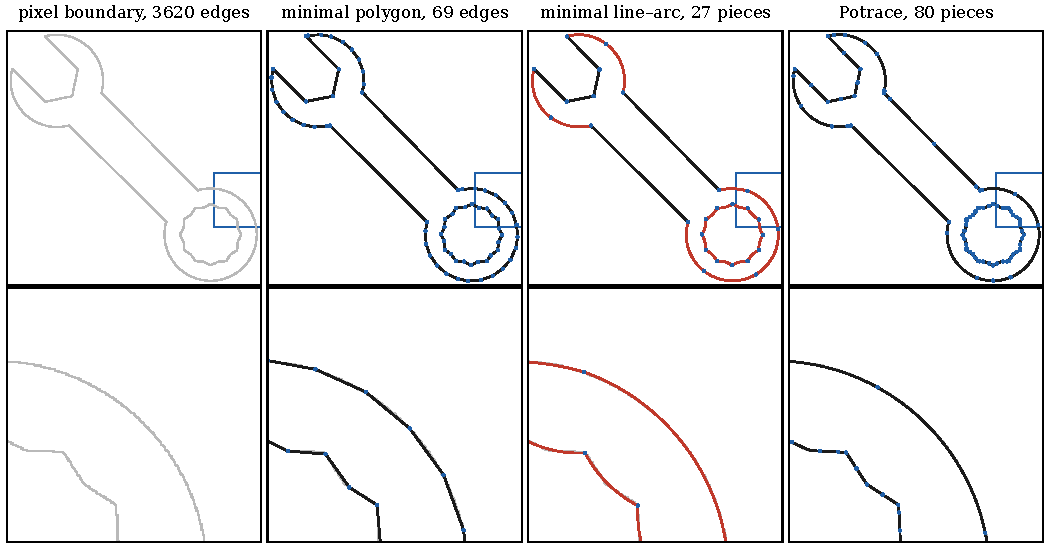
\includegraphics[width=\linewidth]{figures/fig_models.pdf}
\caption{One input at $\varepsilon=2$ (grey: pixel boundary, $3620$ edges;
dots: piece end points; red: circular arcs). The minimal polygon, the minimal
line--arc ring and Potrace's default output use $69$, $27$ and $80$ pieces.
The first two are certified; the bottom row enlarges the marked square.}
\label{fig:models}
\end{figure}

\paragraph{Where the time goes.} The certificate is not the expensive part.
Per input, the median time of the strict certified re-selection, which may
certify several candidates, is $5$--$7$\,s; the joint minimal polygon takes
about $1$\,s; and the line--arc search takes $74$\,s at $\varepsilon=1$ and
$24$--$27$\,s otherwise, that is $64$--$78\%$ of the analysis. The cost of the
method is therefore the cost of proving optimality, not of proving the error
bound, and a model produced by any other means can be certified at the lower
price (Section~\ref{sec:audit}): on Potrace's output the checker alone takes
a median $3.0$\,s per input, in Python and without any tuning.

\paragraph{How much of the time is the language.} The implementation is
NumPy code, and Potrace is optimised C, so the comparison of
Table~\ref{tab:potrace} mixes the cost of the method with the cost of the
language. To separate them we rewrote the dominant kernel of the line--arc
search, the computation of the admissible pairs of
Proposition~\ref{prop:interval} for all node pairs of a ring, as a plain
scalar loop in a compiled language (C\#, .NET Framework~4 just-in-time
compiler, one thread, no vector instructions), and ran both versions on all
rings of six icons (Table~\ref{tab:kernel}). This comparison was made with an
earlier version on bitmaps resampled to a $1000$-unit plane and was not
repeated; it concerns the kernel, not the inputs.

\begin{table}[h]
\centering
\caption{The admissible-pair kernel of the line--arc search on the 34 rings
of six icons ($103\,232$ dense nodes): vectorised NumPy against a scalar
compiled loop. The two versions return identical sets.}
\label{tab:kernel}
\begin{tabular}{rrrrrr}
\toprule
$\varepsilon$ & admissible pairs & differing & NumPy (s) & compiled (s) & factor\\
\midrule
1 & 4\,501\,914 & 0 & 697.5 & 104.7 & 6.7\\
2 & 21\,565\,138 & 0 & 149.5 & 25.6 & 5.8\\
5 & 15\,612\,681 & 0 & 111.8 & 20.8 & 5.4\\
\bottomrule
\end{tabular}
\end{table}

The compiled loop is $5.4$ to $6.7$ times faster and reproduces the NumPy
result on every one of the $4.2\cdot10^{7}$ admissible pairs. This is a
measured lower bound on what a port would gain, not an estimate of a tuned
implementation: the loop is independent across node pairs, so it
parallelises trivially, and neither threads nor vector instructions were
used. It also shows what a port would not change. Even six times faster, the
line--arc search would take seconds to tens of seconds per icon, three orders
of magnitude more than Potrace; the gap is the price of testing every node
pair rather than committing greedily, and only a better pruning of pairs, not
a faster language, would close it. The minimal polygon and the certificate
were not ported.

\paragraph{Size of the certificate.} No proof object is stored. The checker
re-derives every bound from the stored coefficients and the reference
boundary, so the certificate adds only a record of its outcome: about
$0.8$\,kB per project in the three inputs we measured, next to $38$--$66$\,kB
for the selected model and $40$--$73$\,kB for the reference boundary in the
same uncompressed JSON encoding. The only stored witness is the removal
sequence of Theorem~\ref{thm:triangle}, which is linear in the number of
removed vertices.

\subsection{Sensitivity to the cost model and to families}\label{sec:costablation}

\emph{Cost model.} Re-selecting among the same candidates with
\texttt{mdl\_v1} instead of \texttt{fixed64\_v1} leaves the selection
unchanged on $200$, $172$, $163$ and $143$ of the 200 inputs for
$\varepsilon=1,2,3,5$. Under \texttt{mdl\_v1} the line--arc ring is selected
on $136$, $137$, $128$ and $118$ inputs and the minimal polygon on $3$, $5$,
$11$ and $32$, with median code lengths $1522.5$, $1349$, $1299.5$ and
$1280.5$ bits. The two cost models disagree mainly at loose tolerances, where
\texttt{mdl\_v1} charges a line $2$ reals instead of $6$ and therefore
prefers polygons more often.

\emph{Families.} Removing one family from the recorded accepted candidates and
re-solving gives the price of that family under \texttt{mdl\_v1}. Without the
line--arc ring the best accepted cost rises by a mean factor
$1.03$--$1.05$ (maximum $2.47$); without the per-ring hybrid by
$1.09$--$1.11$ (maximum $4.33$); without the minimal polygons by $1.22$ at
$\varepsilon=1$, entirely because of two inputs with contacts on which it is
the only compact certified candidate (maximum $36$), and by at most $1.01$
otherwise. These factors are small because the hybrid combines, ring by
ring, the cheapest accepted pieces of all families and therefore itself
contains rings of the removed family; they are lower bounds on a family's
contribution. The ablation uses the measured acceptance test, not
certificates.

\subsection{Independent measurement of Potrace}\label{sec:audit}

Potrace~1.16 was run on the same bitmap, so that both methods see the same
$\Gamma$. Its SVG output was flattened to $0.005$ pixels with the standard
second-difference bound and measured with Lemma~\ref{lem:sampling}
($h=0.25$) on the union of all rings, which requires no ring matching and
favours Potrace. Component and hole counts were derived from the flattened
rings. These measurements are floating-point, not certified.

\begin{table}[h]
\centering
\caption{Potrace~1.16 on the 2050 icons. ``$\le\varepsilon$'' counts inputs
whose measured upper bound is within the tolerance; ``topology'' counts inputs
with the reference component and hole counts; ``crossing'' counts outputs with
a non-simple ring or intersecting rings.}
\label{tab:potrace}
\begin{tabular}{lrrrrrrrr}
\toprule
setting & median & median & max & $\le1$ & $\le2$ & $\le3$ & topology & crossing\\
 & pieces & error & error & & & & & \\
\midrule
default & 56 & 1.55 & 7.18 & 4 & 1922 & 2025 & 1950 & 70\\
\texttt{-t 0} & 56 & 1.55 & 7.18 & 4 & 1923 & 2027 & 1952 & 70\\
\texttt{-t 0 -a 0} & 254 & 1.07 & 1.33 & 522 & 2050 & 2050 & 1960 & 62\\
\bottomrule
\end{tabular}
\end{table}

Potrace has no error parameter. With curve smoothing its error exceeds one
pixel on all but four inputs and two pixels on about $6\%$; in polygon-only
mode it stays below $1.34$ pixels but uses $254$ pieces where the certified
minimum for $\varepsilon=1$ is $118$ edges, or $36$ line--arc pieces on the
sample. In every setting $4.4$--$4.9\%$ of the outputs differ from the
reference in component or hole count. Potrace is three to four orders of
magnitude faster (median $0.02$--$0.03$\,s per input) than the present Python
implementation; the comparison concerns guarantees, not speed.

\paragraph{Certifying a third-party tracer.} The checker needs only a model
and the reference boundary, so it can be attached to the output of a tool
that offers no guarantee. We converted Potrace's default output on the 2050
icons to line and cubic B\'ezier pieces, matched its rings to the reference
rings by a minimum-cost assignment on sampled distances, aligned their
orientation and ran the same checker ($h=0.25$, $\delta=0.005$). On $29$
inputs Potrace returns a different number of rings and no matching exists.
On the other $2021$ the error bound is certified, with median $1.55$ pixels,
and the topology is proven on $1973$; it remains undetermined on $48$, four of
which have point contacts. A proven model within $1$, $2$, $3$ and $5$ pixels
is obtained on $4$, $1859$, $1950$ and $1956$ inputs. The certificate takes a
median $3.0$\,s per input against $0.03$\,s for Potrace itself. Thus about
$91\%$ of Potrace's outputs are correct to two pixels and can be proven so
after the fact; what the optimisation of this paper adds is the guarantee in
advance, a prescribed tolerance, and a minimal number of pieces. The same
audit accepts the SVG output of any tracer that is run on the bitmap
(\texttt{examples/certify\_svg.py}: lines, quadratic and cubic B\'ezier
pieces, the usual path commands and transforms). We applied it to Potrace
only; perception-driven and learned
vectorisers~\cite{hoshyari2018,dominici2020,rodriguez2025} were not run, so
this paper contains no measurement of their error or of their topology.

\subsection{What resampling does to the topology}\label{sec:resampling}

Tracing tools commonly rescale the input before tracing, and so did earlier
versions of this implementation, which resampled the thresholded bitmap to a
$1000\times1000$ plane with nearest-neighbour interpolation. A certificate
computed after that step refers to the resampled bitmap. We counted
components, holes and point contacts before and after it
(Table~\ref{tab:resampling}). For the icons, which are scaled by $0.96$, the
counts change on $7$ of the 2050 inputs: a thin gap closes or a thin bridge
opens. For a contour-like input the damage is still small at a scale of
$0.23$, but a drawing made of thin strokes is shredded: at $4096^2$ its $256$
components become $2961$ and its $9$ contact points $2157$. A guarantee about
the resampled image is then a guarantee about a different shape. For this
reason the implementation now works at the resolution of the input by
default and offers the fixed plane only as an option.

\begin{table}[h]
\centering
\caption{Effect of nearest-neighbour resampling to a $1000\times1000$ plane
on the topology of the thresholded bitmap. The large inputs are those of
Section~\ref{sec:scale}.}
\label{tab:resampling}
\begin{tabular}{lrrrrrrr}
\toprule
 & & \multicolumn{2}{c}{components} & \multicolumn{2}{c}{holes} & \multicolumn{2}{c}{contacts}\\
input & scale & before & after & before & after & before & after\\
\midrule
terrain $2048^2$ & 0.47 & 9 & 9 & 4 & 4 & 0 & 0\\
terrain $4096^2$ & 0.23 & 52 & 53 & 30 & 30 & 0 & 1\\
drawing $2048^2$ & 0.47 & 64 & 145 & 57 & 51 & 2 & 86\\
drawing $4096^2$ & 0.23 & 256 & 2961 & 216 & 68 & 9 & 2157\\
\bottomrule
\end{tabular}
\end{table}

\subsection{Large inputs at native resolution}\label{sec:scale}

The icons are one megapixel each. To see how the method behaves on large
rasters we ran boundary tracing, the joint minimal polygon, the minimal
line--arc ring and the checker on inputs of up to $67$ megapixels, with the
tolerance in source pixels as before. Two seeded
synthetic families are used:
\emph{terrain}, the super-level set of a smoothed random field with a fixed
feature size, which resembles a contour map and whose boundary length grows
with the area; and \emph{drawing}, a grid of thick strokes, circles and
rounded rectangles, which resembles a scanned technical drawing and contains
point contacts. Apart from the single scanned map reported at the end of this
subsection, no real maps or scans were used.

Three fixed resource limits of the implementation had to be lifted for this
experiment: the tracer refused more than $4\cdot10^{5}$ unit edges, the
topology check of Corollary~\ref{cor:isotopy} returned \emph{undetermined}
above $5\cdot10^{4}$ leaves because it compared all pairs of bounding boxes,
and the Hausdorff check refused more than $5\cdot10^{5}$ samples per ring.
The pairwise comparison was replaced by a spatial index that yields the same
candidate pairs, and the two other limits became parameters.

\begin{table}[h]
\centering
\caption{Terrain inputs at native resolution, joint minimal polygon,
$\varepsilon=1$ source pixel. All four results are optimal in the admissible
class and proven by the checker. Times are single-threaded and were measured
while other experiments were running; repeated runs differed by up to
$60\%$.}
\label{tab:scale}
\begin{tabular}{rrrrrrr}
\toprule
size & megapixels & reference & rings & edges & search & certificate\\
 & & edges & & & (s) & (s)\\
\midrule
$1024^2$ & 1.0 & 5\,720 & 12 & 418 & 1.3 & 1.7\\
$2048^2$ & 4.2 & 19\,952 & 13 & 1\,396 & 4.3 & 5.8\\
$4096^2$ & 16.8 & 90\,432 & 82 & 6\,155 & 20.9 & 37.5\\
$8192^2$ & 67.1 & 370\,558 & 285 & 25\,184 & 78.7 & 169.2\\
\bottomrule
\end{tabular}
\end{table}

\begin{figure}[t]
\centering
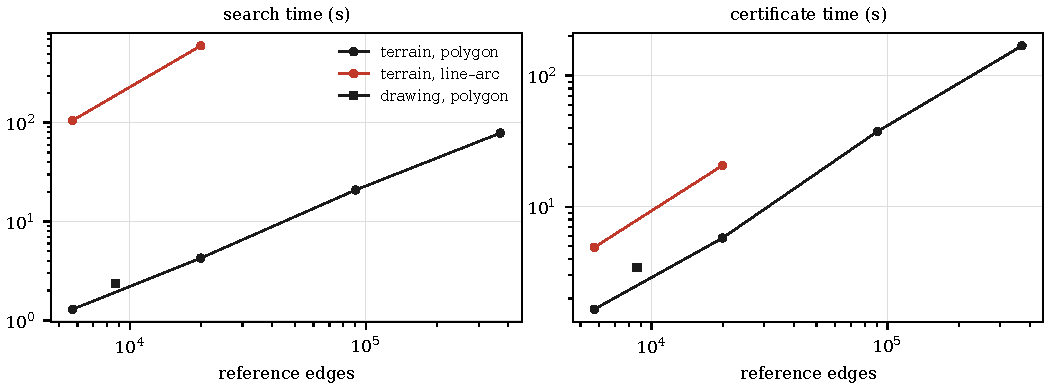
\includegraphics[width=\linewidth]{figures/fig_scale.pdf}
\caption{Search and certificate time against the number of reference edges
at $\varepsilon=1$; only runs that are optimal in their class and proven are
shown.}
\label{fig:scale}
\end{figure}

On terrain inputs the polygon path scales to $67$ megapixels
(Table~\ref{tab:scale}, Figure~\ref{fig:scale}): the search time grows by a
factor $60$ while the reference grows by a factor $65$, and the certificate
by a factor $100$. At $\varepsilon=2$ the same inputs need $240$, $779$,
$3440$ and $14\,025$ edges and are again optimal and proven. The line--arc
ring needs $172$ and $576$ pieces at $1024^2$ and $2048^2$, about $41\%$ of
the polygon, and is optimal and proven, but its search takes $106$\,s and
$601$\,s, two orders of magnitude more than the polygon; we did not run it on
larger inputs.

The drawing inputs expose the limit of the joint search. At $1024^2$ (one
contact point) the minimal polygon is found and certified in $2.3$\,s at
$\varepsilon=1$ and in $158$\,s at $\varepsilon=2$. At $2048^2$ (two contact
points, $121$ rings) the search did not prove an optimum within $3000$ outer
nodes, ten times the default, after $36$ minutes, and larger sizes were not
attempted. The line--arc ring, which is solved ring by ring, is optimal in
its class at $1024^2$ and $2048^2$ ($224$ and $802$ pieces, in $260$\,s and
$2131$\,s), but its topology is undetermined, because it does not preserve
the contacts. Dense
strokes with contacts are therefore outside what the present search handles
at scale.

\paragraph{One scanned map.} As a single observation on real data we took
a $1024\times1024$ crop of a scanned topographic sheet (U.S. Geological
Survey, Santa Cruz quadrangle, 1902; public domain) and thresholded it with
Otsu's method. The result has $6223$ rings, $146\,442$ reference edges and
$2274$ point contacts, most of them produced by scanner noise and by
touching contour lines. The joint search reached the default node limit
after $37$ minutes at $\varepsilon=1$ and $15$ minutes at $\varepsilon=2$
without an admissible family, and the relaxed family it returns is not
certified. This is one crop of one document and not an evaluation, but it
shows the present limit plainly: on noisy scans the number of contacts, not
the number of pixels, decides whether the optimum can be proven, and a scan
would have to be cleaned first, which changes the reference.

\subsection{Colour images by stacked layers}\label{sec:color}

The method is defined for a binary image. A flat-colour image with labels
$0,\dots,K-1$ reduces to $K-1$ binary problems: for $k\ge1$ let
$L_k$ be the set of pixels with label at least $k$, vectorise each $L_k$
independently, and paint the models in the order $k=1,\dots,K-1$ over a
background of colour~$0$. No gaps can appear between neighbouring regions,
because every layer covers all layers painted after it, and each layer
carries its own certificate. The order of the labels is arbitrary; for a
hypsometric map the natural order makes every $L_k$ a super-level set.

We applied this to a six-colour terrain map
(Figure~\ref{fig:color}). At $2048^2$ the five layers have $88\,010$
reference edges; the minimal polygons use $6358$ edges at $\varepsilon=1$ and
$3590$ at $\varepsilon=2$, every layer is optimal in its class and proven,
and search and certificates take $23$\,s and $24$\,s in total at
$\varepsilon=1$. At $4096^2$ ($377\,626$ reference edges) the result is
$26\,545$ edges, again optimal and proven on every layer, in $211$\,s and
$357$\,s. Rasterising the painted model at pixel centres and comparing it
with the input label by label, $0.61\%$ of the pixels differ at
$\varepsilon=1$ ($0.64\%$ at $4096^2$) and $1.86\%$ at $\varepsilon=2$, and
every differing pixel centre lies within $0.52$ and $1.51$ pixels of a layer
boundary respectively. This agreement is measured, not certified: the
certificate bounds the distance between boundaries, and we have not proven
that it implies equal labels away from them. Photographs and images with
gradients are outside the scope; they would first have to be quantised, and
the quantisation error is not covered by any statement of this paper.

\begin{figure}[t]
\centering
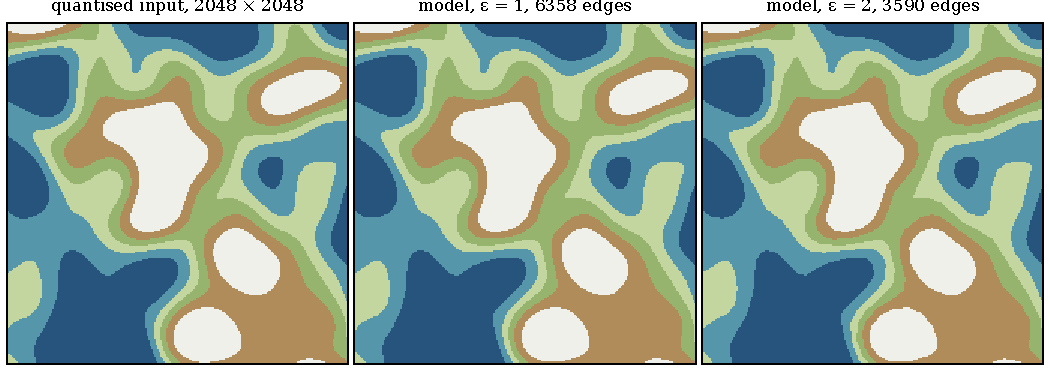
\includegraphics[width=\linewidth]{figures/fig_color.pdf}
\caption{A crop of the six-colour terrain map at $2048^2$ and of the painted
stacked-layer models. Every layer is a certified minimal polygon.}
\label{fig:color}
\end{figure}

\section{Scope and limitations}\label{sec:scope}

The method is meant for settings in which a stated error bound and an
unchanged topology are worth computation time: CAD exchange, manufacturing,
metrology and archival of line art. It is not a replacement for a fast
tracer in graphic design, and it makes no claim outside the following
boundaries.

\paragraph{What is optimised.} The objective is a description cost under a
Hausdorff constraint and a topology constraint. Two models with the same
error and the same number of pieces are equivalent for this objective and
may differ visibly. In particular the line--arc ring is only continuous: no
tangent continuity is imposed at the joints, and no smoothness or perceptual
term enters the cost. Re-choosing the bulges inside their admissible
intervals reduces the corners only marginally
(Section~\ref{sec:arc-results}), because the nodes of a minimal ring were not
chosen for smoothness. A tangent-continuous optimum is a different problem:
the cost of a piece then depends on its neighbours, so the shortest-cycle
argument, which needs independent pieces, no longer applies, and the natural
replacement is a shortest path over pairs of consecutive pieces with the
tangent direction as additional state. For CAD use this is the most
important missing piece. No user study has been carried out, so nothing is
claimed about visual quality.

\paragraph{What is optimal.} Minimality is proven for two families,
node-restricted polygons and node-restricted line--arc rings, and is
relative to the node set; for line--arc rings also to the span limit, and it
is computed ring by ring without the contact and clearance constraints, so
that the ring is rejected on inputs with point contacts. Pinning the contact
points is as easy for arcs as for chords (Lemma~\ref{lem:pin}), but
Theorem~\ref{thm:contact} is proven for polygonal models only: its conditions
(1) and (3) would have to be replaced by exact intersection and
tangent-order tests between circular arcs, which are decidable in rational
arithmetic for arcs with rational centres but are not implemented, and the
clearance constraint would need the blocking sets of
Proposition~\ref{prop:block} for arcs. On the 41 icons with contacts the
joint minimal polygon therefore remains the certified answer. A different family
may describe the same shape with fewer pieces. For B\'ezier, B-spline and
conic families the pipeline remains a bounded candidate search without any
optimality statement.

\paragraph{Cost and scale.} The certificate is cheap relative to the search
(Section~\ref{sec:costablation}), but the implementation as a whole is slow:
a median of $31$--$115$\,s per icon against $0.03$\,s for Potrace. The joint
search has no polynomial bound and is not an anytime algorithm
(Section~\ref{sec:constrained}): two of the 8200 icon instances exceed the
default node limit, and on a dense $2048\times2048$ drawing with contacts and
on a crop of a scanned map no optimum was proven (Section~\ref{sec:scale}).
The polygon path was run up to $67$ megapixels on contour-like inputs; the
line--arc search was not run beyond four megapixels, and its optimum depends
on the span limit (Table~\ref{tab:span}). The large and colour inputs of this
paper are synthetic, and no systematic evaluation on scanned documents or on
noisy rasters was carried out.

\paragraph{Input model.} The input is a binary image, or a flat-colour image
treated as stacked binary layers (Section~\ref{sec:color}). Photographs,
gradients and anti-aliased edges are not addressed. Errors are measured
against the pixel boundary, not against an ideal continuous shape, and the
topology of the pixel boundary is preserved exactly: a speck of noise or a
pinhole in a scan is kept, even where an application would prefer to remove
it. The primary dataset consists of icons rendered from vector sources.

\paragraph{Nature of the guarantee.} The topology conditions are sufficient
and may return \emph{undetermined}. The certificate is an executable checker
under Assumption~\ref{ass:ieee}, not a machine-checked proof. The work
concerns planar boundaries; surfaces, solids and boundary representations of
three-dimensional CAD are out of scope, and the method has not been
evaluated inside a production CAD or illustration system.


\section{Code and data availability}\label{sec:availability}

% If the venue is double-blind, replace the two links by an anonymised mirror.
The implementation (release 3.0.0, MIT licence), the experiment scripts, the
dataset manifest and the recorded results of every table are available at
\url{https://github.com/Hakan-karateke/certified-vectorization} and archived at
\url{https://doi.org/10.5281/zenodo.24299983}. The numbers of
this paper are produced by the following scripts in \texttt{examples/}:
\begin{itemize}
\item \texttt{optimality\_gap.py}: Table~\ref{tab:gap} and
  Section~\ref{sec:constrained-results};
\item \texttt{line\_arc\_optimum.py}: Table~\ref{tab:arcs};
\item \texttt{line\_arc\_sensitivity.py}: Table~\ref{tab:span}, tangent
  smoothing and the clearance study;
\item the sweep of \texttt{sekilden\_denkleme.stress} with
  \texttt{summarize\_sweep.py}: Table~\ref{tab:pipeline} and
  Section~\ref{sec:costablation};
\item \texttt{compare\_potrace.py}, \texttt{certify\_potrace.py} and
  \texttt{certify\_svg.py}: Section~\ref{sec:audit};
\item \texttt{scan\_degradation.py} (subcommand \texttt{resample}):
  Table~\ref{tab:resampling}; \texttt{real\_scans.py}: the scanned map of
  Section~\ref{sec:scale};
\item \texttt{native\_inputs.py}: Sections~\ref{sec:scale}
  and~\ref{sec:color};
\item \texttt{compiled\_kernel/compare.py}: Table~\ref{tab:kernel};
\item \texttt{paper/make\_figures.py}: all figures.
\end{itemize}
The icon set is Bootstrap Icons~1.11.3 under the MIT licence; the manifest
records the archive hash, the rasteriser versions and a SHA-256 digest of
every rendered bitmap, and the large and colour inputs are regenerated from a
fixed seed. The scanned map is not redistributed; its source and digest are
recorded with the results. Potrace~1.16 is used unmodified. The whole icon
study is run by \texttt{examples/run\_all\_experiments.sh}. The test suite
(225 tests)
includes the counterexample of Remark~\ref{rem:necklace}, brute-force
comparisons for both minimal families and an independent distance
computation for Proposition~\ref{prop:interval}.


\appendix
\section{Proof of Theorem~\ref{thm:contact}}\label{app:contact}

Throughout, the plane is oriented and regarded as the sphere $S^2$ minus the
point $\infty$. The pixel boundary $\Gamma$ itself satisfies conditions (1)
to (3): its edges are distinct unit lattice edges, so two rings, or two parts
of one ring, can only meet at lattice points, which are then repeated nodes
and belong to $K$; and at such a point the four rays are the four lattice
directions.

\begin{lemma}\label{lem:planegraph}
Under conditions (1) to (3) the arcs of $M$ between consecutive contact points
are simple polygonal paths, two different arcs meet only at common end points
in $K$, and a ring without contact points is a simple closed polygon disjoint
from all other rings. Hence $\Gamma$ and $M$ are embeddings in the plane of
the same abstract graph, with vertex set $K$, the arcs corresponding by ring
and position in the contact sequence.
\end{lemma}
\begin{proof}
Two consecutive edges of a ring share one vertex and, not folding back, meet
only there. Two non-consecutive edges are disjoint by (3) unless they end at
a common point $k\in K$; in that case they are two rays from $k$ with
different directions by (2), so they meet only at $k$. Interior vertices of
an arc are not in $K$ and are not repeated by (1). Therefore an arc does not
meet itself, and two arcs meet only at points of $K$ that are end points of
both. The correspondence of arcs is condition (1).
\end{proof}

\begin{lemma}\label{lem:sphere}
For every connected component $C$ of the graph there is an
orientation-preserving homeomorphism $h_C$ of $S^2$ that maps every arc of
$\Gamma_C$ onto the corresponding arc of $M_C$ with the same direction. It
maps the face on a given side of an arc of $\Gamma_C$ to the face on the same
side of the corresponding arc of $M_C$.
\end{lemma}
\begin{proof}
If $C$ has a vertex, $\Gamma_C$ and $M_C$ are embeddings of a connected graph
in the sphere; such embeddings are cellular, and by (2) they have the same
rotation system, the rays being matched by ring, pass and direction. Two
cellular embeddings of a connected graph in an oriented surface with the same
rotation system differ by an orientation-preserving homeomorphism of the
surface that respects the edges~\cite[Section~3.2]{mohar2001}; the labels fix
the direction of every arc. If $C$ is a single ring without contact points,
both curves are Jordan curves and the Schoenflies theorem gives a
homeomorphism of $S^2$ between them, which can be chosen orientation
preserving and direction preserving after composing, if necessary, with a
half-turn of the sphere that maps the curve to itself and exchanges its two
sides. The last statement holds because $h_C$ preserves the orientation of
the sphere and the direction of the arc.
\end{proof}

By Lemma~\ref{lem:sphere} the set of sides bounding a face is the same for
corresponding faces, which justifies naming a face by one of its sides.
Condition (4) now reads: $h_C$ maps the face of $\Gamma_C$ containing $\infty$
to the face of $M_C$ containing $\infty$, and the face containing $\Gamma_D$ to
the face containing $M_D$.

We use two classical facts. \emph{Janiszewski's theorem}: if $A,B\subset S^2$
are compact, $A\cap B$ is connected or empty, and neither $A$ nor $B$
separates two points, then $A\cup B$ does not separate
them~\cite{newman1951}. \emph{Faces of connected graphs}: every face of a
connected graph embedded in the sphere is simply connected, so its complement
is connected.

For a component $C$ write $\widehat{\Gamma}_C$ for $\Gamma_C$ together with
its bounded faces, and similarly $\widehat{M}_C$.

\begin{lemma}\label{lem:minimal}
If $\Gamma_D$ lies in a bounded face $f$ of $\Gamma_C$, then
$\widehat{\Gamma}_D\subset f$. Consequently a component $D$ for which
$\widehat{\Gamma}_D$ has minimal area contains no other component in its
bounded faces, and the same is then true of $M_D$.
\end{lemma}
\begin{proof}
The complement of $f$ in the sphere is connected, contains $\infty$ and does
not meet $\Gamma_D$; it therefore lies in the unbounded face of $\Gamma_D$,
which gives $\widehat{\Gamma}_D\subset f$ and a strictly smaller area than
$\widehat{\Gamma}_C$. For the last statement, every other component lies in
the unbounded face of $\Gamma_D$, hence by condition (4), applied to the pair
$(D,C)$ and to the unbounded face of $D$, in the unbounded face of $M_D$.
\end{proof}

\begin{lemma}[Relocation]\label{lem:relocate}
Let $W$ be a connected open subset of the plane, let $A,B\subset W$ be
connected polygonal graphs whose bounded faces lie in $W$, and let $\psi$ be
an orientation-preserving homeomorphism of the plane with $\psi(A)=B$. Then
there is an orientation-preserving homeomorphism $\varphi$ of the plane that
is the identity outside a compact subset of $W$ and agrees with $\psi$ on $A$.
\end{lemma}
\begin{proof}
Write $\widehat{A}$ for $A$ together with its bounded faces. The sets
$\widehat{A}$ and $\widehat{B}$ are compact, polygonal, connected and have
connected complement, so each has arbitrarily small closed polygonal disc
neighbourhoods. Choose such a disc $N_B\subset W$ around $\widehat{B}$ and
then a disc $N_A\subset W$ around $\widehat{A}$ so small that
$\psi(N_A)\subset\operatorname{int}N_B$.

\emph{Step 1.} There is an orientation-preserving homeomorphism $\theta$ of
the plane, the identity outside a compact subset of $W$, with
$\theta(N_A)\subset\operatorname{int}N_B$: first shrink $N_A$, inside a
slightly larger disc contained in $W$, to a small disc around one of its
points, and then push this small disc along a polygonal path in the connected
set $W$ to a point of $\operatorname{int}N_B$, by a homeomorphism supported
in a thin neighbourhood of the path.

\emph{Step 2.} Put $N_1=\theta(N_A)$ and $\psi_1=\psi\circ\theta^{-1}$, so
that $\psi_1$ preserves orientation, maps $\theta(A)$ onto $B$, and
$\psi_1(N_1)=\psi(N_A)\subset\operatorname{int}N_B$. By the Schoenflies
theorem $N_B\setminus\operatorname{int}N_1$ and
$N_B\setminus\psi_1(\operatorname{int}N_1)$ are closed annuli. Define
$\varphi_1=\psi_1$ on $N_1$, the identity outside $N_B$, and on the first
annulus a homeomorphism onto the second that extends $\psi_1$ on
$\partial N_1$ and the identity on $\partial N_B$; it exists because both
boundary maps preserve orientation. Then $\varphi=\varphi_1\circ\theta$ is
the identity outside a compact subset of $W$ and equals $\psi$ on $A$.
\end{proof}

\begin{proof}[Proof of Theorem~\ref{thm:contact}]
We show by induction on the number of components in a set $S$ that there is
an orientation-preserving homeomorphism $g_S$ of the plane mapping every arc
of $\Gamma_C$, $C\in S$, onto the corresponding arc of $M_C$ with the same
direction. The theorem is the case of all components.

\emph{One component.} By condition (4), $h_C(\infty)$ lies in the unbounded
face of $M_C$. This face is open and connected, so there is a homeomorphism of
the sphere, the identity outside a compact subset of the face, that moves
$h_C(\infty)$ to $\infty$. Composing gives $g_{\{C\}}$.

\emph{Induction step.} Let $D\in S$ be as in Lemma~\ref{lem:minimal}, let
$S'=S\setminus\{D\}$, $g=g_{S'}$, and $M'=\bigcup_{C\in S'}M_C$. Put
$A=g(\Gamma_D)$. For every $C\in S'$ the sets $A$ and $M_D$ lie in the same
face of $M_C$: the map $g$ preserves orientation and the direction of the
arcs of $\Gamma_C$, so it maps the face of $\Gamma_C$ containing $\Gamma_D$ to
the face of $M_C$ bounded by the same sides, which contains $M_D$ by
condition (4). The sets $M_C$, $C\in S'$, are compact and pairwise disjoint,
so by Janiszewski's theorem, applied repeatedly, $M'$ does not separate a
point of $A$ from a point of $M_D$: both lie in one face $W$ of $M'$. The
bounded faces of $A$ are the images of those of $\Gamma_D$ and contain no
point of $M'$; the bounded faces of $M_D$ contain no point of $M'$ by
Lemma~\ref{lem:minimal}; each of these faces together with its boundary is a
connected set in the complement of $M'$ that meets $W$, so it lies in $W$.

Let $\psi$ be the homeomorphism obtained from the case of one component for
$D$, composed with $g^{-1}$: it preserves orientation and maps $A$ onto $M_D$
arc by arc. Lemma~\ref{lem:relocate} gives $\varphi$, the identity outside a
compact subset of $W$ and hence on $M'$, that agrees with $\psi$ on $A$. Then
$g_S=\varphi\circ g$ has the required property.
\end{proof}

\bibliographystyle{plain}
\bibliography{references}

\end{document}
